\documentclass[12pt]{article}

% TEMPLATE DEFAULT PACKAGES
\usepackage{amssymb,amsmath,amsfonts,eurosym,geometry,ulem,graphicx,color,setspace,sectsty,comment,natbib,pdflscape,array,adjustbox}

% ADDED PACKAGES FOR THIS MANUSCRIPT
\usepackage{palatino,newtxmath,multirow,titlesec,threeparttable,tabu,booktabs,titlesec,threeparttable,mathtools,bm,bbm,subcaption,pdflscape,tcolorbox,mathrsfs,float}
% endfloat,

%\usepackage{kbordermatrix}% http://www.hss.caltech.edu/~kcb/TeX/kbordermatrix.sty
%\usepackage{amsmath}% http://ctan.org/pkg/amsmath

\usepackage{afterpage}
\usepackage[hyphens]{url}
\usepackage[margin=1cm]{caption}

\usepackage[draft]{hyperref}
\newcommand{\tim}{$\,\times\,$}
% FIGURES & TABLES CAPTION STYLING
\captionsetup[figure]{labelfont={bf},name={Figure},labelsep=period}
\captionsetup[table]{labelfont={bf},name={Table},labelsep=period}

% SECTION TITLE SETTINGS
\titlelabel{\thetitle.\enskip}
\titleformat*{\section}{\large\bfseries}
\titleformat*{\subsection}{\normalsize\bfseries}

% COLUMN TYPES
\newcolumntype{L}[1]{>{\raggedright\let\newline\\\arraybackslash\hspace{0pt}}m{#1}}
\newcolumntype{C}{>{\centering\arraybackslash}p{5.2em}}
\newcolumntype{D}{>{\centering\arraybackslash}p{5em}}
\newcolumntype{R}[1]{>{\raggedleft\let\newline\\\arraybackslash\hspace{0pt}}m{#1}}


% MARGINS AND SPACING
\normalem
\geometry{left=1.1in,right=1.1in,top=1.0in,bottom=1.0in}
\setlength{\parskip}{2.5pt}

% SPECIAL CELL 
\newcommand{\specialcell}[2][c]{%
	\begin{tabular}[#1]{@{}l@{}}#2\end{tabular}}

% NO INDENT ON FOOTNOTES
\usepackage[hang,flushmargin]{footmisc}

\begin{document}

\begin{titlepage} 
%\title{{Borrowing with Unpaid Bills}\thanks{}}
\title{{Borrowing with Unpaid Bills}}
\author{\\[3em]
  William Violette\thanks{Federal Trade Commission, Washington, DC. E-mail: william.j.violette@gmail.com   Any opinions and conclusions expressed herein are those of the author and do not necessarily represent the views of the Federal Trade Commission or its Commissioners.} \\
 \\ 
  }
\vspace{30mm}
\date{\vspace{5mm}This Version: \today}
\maketitle
\begin{abstract}

% By tolerating large quantities of unpaid bills each month, public utilities offer an important source of low-cost credit to low-income households.  
%With billing data from piped water in Manila, this paper documents that .. HARD TO GET A CLEAN FACT ABOUT THE CREDIT OFFERED THROUGH UNPAID BILLS
% WORTH GETTING INTO WATER PROVIDERS AS GREAT CREDITORS??  WOULD BE NICE TO HIGHLIGHT THE TRADE-OFF...
% Public utilities often tolerate large amounts of unpaid bills each month.  

Unpaid utility bills may provide an important source of credit to households.  With billing data from a water utility in Manila, Philippines, this paper builds a consumption and savings model to estimate demand for both water and credit.  Estimates suggest that households value billing flexibility from the water utility as much as 8
\unskip\% of an average water bill.  I then analyze the welfare effects of popular proposals to reduce delinquency by requiring upfront payments.  Simulations find that upfront payments do not produce enough cost savings to justify their negative impacts on household consumption smoothing.

%are unable to recoup enough revenue to compensate for their negative effects on household consumption smoothing.

%Simulations imply that these policies reduce social welfare because they are not able to recoup enough revenue to compensate for their negative impacts on household consumption smoothing.


% Estimates suggest that payment flexibility is worth 8
\unskip\% of an average water bill to households. 

% credit as well as borrowing costs  household 

%measure borrowing costs facing households as well as their demand for credit.
%measure how much households value delaying their bill payments.  
%Estimates suggest that households would require an 8\% discount on their water bills in order to commit to always paying  on time.  
% Unpaid bills may provide an important source of credit to households.  With billing data from a piped water provider in Manila, Philippines, this paper estimates a consumption and savings model to measure 
% the welfare effects of requiring immediate payment.
% households would require an 8\% discount on their water bills in order to commit to always paying  on time.  
%I also evaluate the welfare effects of implementing prepaid metering --- a popular proposal to eliminate delinquency.  Simulations imply that this technology would be welfare reducing because installation costs and costs to consumers of outweigh benefits of recovering unpaid bills.   
% This framework also provides a method to estimate credit constraints with utility billing data.  probably don't sell this
% and evaluate the welfare effects of a popular proposal to eliminate delinquency.  I find that households are willing to pay an 8\% premium on their water bill to have bill flexibility.  Implementing prepaid ....

\vspace{2in}
\textbf{Keywords:} credit constraints; consumption smoothing; water utilities. \\
\textbf{JEL Codes:} O13; E21; L95. \\
\bigskip
\end{abstract}
\setcounter{page}{0}
\thispagestyle{empty}
\end{titlepage}
\pagebreak \newpage

%\spacing{1.5}
\onehalfspacing

\section{Introduction}

Households face a dynamic problem of how to smooth their consumption over time, especially in low-income settings where households have little access to formal credit and risky income streams (\cite{morduch1995income}).  Households often resort to costly money lenders or informal arrangements with family members (\cite{banerjee2007economic}).  Firms may provide an additional channel for consumption smoothing by allowing households to delay their payments for goods and services.  In particular, public utilities often tolerate high levels of unpaid bills each month.  Unpaid bills provide an economically important source of credit for households since public utilities cover broad populations and take up at least 5\% of household incomes in developing countries.\footnote{\cite{komives2006distributional} find that households spend 1-2\% of their incomes on water and 4\% on electricity.} 

When market failures limit formal lending, public utilities may provide efficient, second-best sources of credit.  First, poor access to collateral often restricts the availability of lending options to low-income households (\cite{jack2016borrowing}).  Public utilities overcome this barrier by threatening disconnection from future service to enforce repayment.  Second, poor infrastructure and mobile populations increase the transaction costs of screening and monitoring debtors, which contribute to high interest rates (\cite{jack2014risk}).  As part of their business practices, public utilities invest in meter reading and billing systems that may lower these transaction costs.  Third, moneylenders and peer-to-peer lending groups often cater to small pools of debtors while public utilities are able to spread default risk across a wide customer base.  Despite these advantages, linking credit to consumption from public utilities creates an inherent inefficiency by incentivizing overconsumption.  For example, households may substitute toward piped water and away from other beverages in months where they are credit constrained.  Since governments actively regulate public utilities, the extent to which public utilities should provide credit remains an open policy question (\cite{laffont2005regulation}).  

Technologies that eliminate delayed payments have recently dominated utility policy discussions.    Both researchers and policymakers recommend new prepaid metering technologies, which require upfront payments before releasing any services, as effective strategies to prevent nonpayment.\footnote{\cite{kojima2016making} and \cite{heymans2014limits} point to prepaid metering as a successful strategy to reduce nonpayment for electricity and water utilities (respectively).  \cite{jack2016charging} find that prepaid meters for electricity in South Africa substantially increase utility revenues.}    Yet, existing analyses have yet to consider how these technologies may impact household welfare by reducing consumption smoothing.

This paper incorporates delayed payments to public utilities into household consumption and savings decisions in order to evaluate the welfare effects of offering credit through public utilities.  I build a dynamic model where each period, households have the option of borrowing with a costly asset as well as with delayed payments to a public utility.  Low interest rates on delayed payments induce households to increase their borrowing by overconsuming utility services.  The extent to which households value payment flexibility depends on the borrowing costs of other assets, which are often difficult to measure in traditional survey data.

To estimate borrowing costs, I take a structural approach using billing data from a regulated water utility in Manila, Philippines.  The identification strategy leverages months where utility workers visit households and disconnect them if they do not pay their outstanding balances.  If borrowing were costless, households would never be disconnected during these visits because they would pay their outstanding balances with cheap loans.  Therefore, long and frequent disconnections in response to these visits --- especially among households with large outstanding balances --- provide evidence of borrowing costs.  Using this strategy, I estimate high interest rates for borrowing, consistent with poor observed access to formal credit in Manila with only 3.9\% of households having credit cards and 18.7\% having bank accounts.\footnote{Statistics are from the Philippines 2014 Consumer Finance Survey.}  

These estimates also allow me to simulate several counterfactual policies.  First, I find that in a counterfactul where households are required to pay their bills on time (holding all else equal), consumer welfare drops by 50.3
PhP (or 1.5
USD) per household-month, which is equal to 8
\unskip\% of an average water bill.  Usage also declines since households no longer have an incentive to overconsume water to fund their borrowing from unpaid bills.  

Second, I simulate a policy that (1) eliminates delayed payments by charging a high interest rate on unpaid bills, (2) eliminates default risk by preventing households from leaving large outstanding balances when they permanently disconnect, and (3) adjusts prices to ensure that the water utility remains revenue-neutral (consistent with regulation in Manila).\footnote{\cite{laffont2005regulation} discusses economic reasons for these regulatory structures which are common in both developed and developing country settings.}  Without default risk, the utility has fewer costs to recover with prices. Yet without billing flexibility, households use less water, generating less revenue for the utility.  On net, prices remain the same and the policy reduces social welfare by 89.4
PhP (or 2.0
USD) per household-month.  

Finally, I use this framework to evaluate implementing prepaid meters in this context.  While ensuring that households pay upfront, prepaid meters require steep increases in prices to cover their installation and maintenance costs.  As a result, prepaid meters produce large reductions in social welfare on the order of 245.5
PhP (or 5.0
USD) per household-month.  Taken together, these results suggest that popular policies to reduce nonpayment may be welfare reducing primarily by limiting consumption smoothing.  Given around 2.4 million piped water using households in Metro Manila, these policies would imply welfare costs on the order of 32.7
to 144.1
million US dollars per year.

This paper contributes to three main strands of economic literature.  First, this paper brings payment and billing policy questions into a growing literature on optimal policy for utilities in developing countries (\cite{mcrae2015infrastructure}; \cite{szabo2015value}; \cite{jack2016charging}; \cite{jack2015pay}; \cite{szabo2015reducing}).  Building on previous static models, this paper also provides a framework for considering how dynamic incentives affect household demand for public utilities.  Second, this paper draws on a large body of research analyzing household credit constraints, particularly through microfinance interventions (\cite{morduch1999microfinance}; \cite{morduch1995income}; \cite{cull2009microfinance}; \cite{dupas2013savings}; \cite{jack2016borrowing}).  \cite{karlan2009expanding} and \cite{gine2014group} specifically focus on microfinance in the Philippines. Third, \cite{deaton1991saving} provides the foundational model of dynamic decision-making that serves as the starting point for the model in this paper, and the estimation of this model adapts methods developed by \cite{gourinchas2002consumption} and \cite{laibson2007estimating}.

This paper proceeds with Section~\ref{section:data} describing the water billing data from Manila.  Billing practices, disconnection policies, and institutional details are discussed in Section~\ref{section:descriptives} alongside descriptive evidence.  Section~\ref{section:model} develops a model of household consumption and savings decisions while Section~\ref{section:estimation} discusses the estimation and results.  Counterfactual exercises and welfare impacts are provided in Section~\ref{section:counterfactuals}.  Section~\ref{section:conclusion} concludes.

\section{Data}\label{section:data}

% Describe notice of disconnection in more detail here??? and  NO DO IT LATER~! PLEASE!!!!

Measuring credit through unpaid water bills requires information on monthly water bills at the household-level.  This paper relies primarily on water utility records collected as part of a research partnership with one of the two regulated utilities in Metro Manila, Philippines where each utility is responsible for serving their assigned geographic half of Metro Manila.  This utility provided access to monthly billing records for each connection as well as detailed information covering the regulatory structure and costs of production.  The monthly billing records include meter readings, billing amount, outstanding balances, and payments spanning January, 2010 to May, 2015.  Over this timeframe, the total number of connections increased from 900,000 to 1,500,000 as the water utility expanded service access.  Water connections are split into four categories: residential (90\%), semi-business (4\%), commercial (5\%), and industrial (1\%).  Since this research focuses on household decisions, only connections coded as residential are included in the analysis.  

Since multiple households often share the same connections in Manila, the billing data is merged to survey data that measures the number of households using each connection as well as demographics for the household that owns the connection.  Conducted every two years between 2008 and 2012, the survey data cover a total of nearly 50,000 water connections.  Connection survey documentation indicates that surveyors used stratified random sampling where the number of connections surveyed was proportional to the census population in the smallest administrative census region, making this survey roughly representative of the population of piped water users.  

Using this survey data, the analysis is further limited to connections that each serve a single household in order to ensure that billing data for each connection maps directly into the consumption and savings decisions of a single household.  Previous research from \cite{wjv} finds that sharing a connection with multiple households increases the costs of consuming water for each household, which affects each household's water demand.  \cite{wjv} also finds that households using a connection individually tend to have higher water demand, larger household sizes, and greater likelihood of living in single houses (as opposed to duplexes or apartments) in comparison to households sharing water connections.  These differences may limit the generalizability of the findings outside of this subpopulation in Manila.  This sample restriction also ensures that household-level data and connection-level data can be referred to interchangeably.  Table~\ref{table:sampleconstruction} in Appendix~\ref{appendix:sampleconstruction} includes more details on how the sample is constructed for the analysis. 

Because the connection survey data does not include income measures, average monthly income for households in Manila is taken from the 2015 Family Income and Expenditure Survey.  The average interest rate for the Philippines is calibrated from the World Bank Databank (2010-2015).

\section{Credit through Unpaid Water Bills}\label{section:descriptives}

% \footnote{The company upgraded t in the first year of the sample.  Previously, the company mailed the bill to each household at the end of the month.} 
% Each month, households consume 24m3 of piped water on average, which totals an average monthly bill of 691.6PhP as shown in Table~\ref{table:descriptives_all}.  Given an average monthly income in Manila of 31,910PhP and savings rate of 5,730PhP,  monthly water bills reach a modest average of 2.2\unskip\% of income and 10.6\unskip\% of savings.  


\begin{table}[h!] % PUT IN DEMOGRAPHICS PLEASE ?!?!?
\centering
\caption{Mean Characteristics}\label{table:descriptives_all}
\vspace{-2mm}
\begin{tabular}{l*{1}{cccccc}}
\toprule
 & Mean & SD & Min & 25th & 75th & Max  \\
\midrule
 Usage (m3)  & 24.9  & 17.0  & 0.0  & 14.0  & 32.0  & 200.0  \\ 
 Bill  & 692  & 927  & -4,640  & 265  & 854  & 78,409  \\ 
 Unpaid Balance  & 1,523  & 4,611  & -4,995  & 0  & 1,126  & 79,904  \\ 
 Share of Months with Payment  & 0.71  & 0.45  & 0.00  & 0.00  & 1.00  & 1.00  \\ 
 Payment Size  & 924  & 1,147  & 0  & 316  & 1,082  & 62,879  \\ 
 Days Delinquent  & 50.2  & 133.6  & 0.0  & 0.0  & 31.0  & 720.0  \\ 
 Delinquency Visits per HH  & 0.42  & 0.71  & 0.00  & 0.00  & 1.00  & 6.00  \\ 
 Share of Months Disconnected  & 0.04  & 0.19  & 0.00  & 0.00  & 0.00  & 1.00  \\ 

\bottomrule \\ [-.8em]
\multicolumn{7}{l}{Total Households: 46,098  Obs. per Household: 60.9 Total Obs.: 2,123,335} \\
\multicolumn{7}{l}{\scriptsize Bill, Unpaid Balance, and Payment Size are in PhP per household-month.  45 PhP $\sim$ 1 USD} \\[-.5em]
\multicolumn{7}{l}{\scriptsize Negative bills and balances generally arise from refunds for billing or payment errors.}  \\[-.5em]
\multicolumn{7}{l}{\scriptsize See Appendix~\ref{appendix:sampleconstruction} for more details on the sample construction.} 
\end{tabular}
\end{table}

Unpaid water bills may provide a reliable source of low-cost credit to households because (1) the utility tolerates high rates of delinquency before disconnecting water service and (2) the utility is prohibited from charging any interest on outstanding balances. 

At the end of each month, the utility sends meter readers who record monthly consumption for each connection and then use a mobile device to print and deliver the bill to households in person.  Households are then expected to pay the bill by the end of the month.  Households have many options to pay their bills with 79\unskip\% using small payment centers (mall kiosks, gas stations, convenient stores, etc.), 9.4\unskip\% paying at local utility offices, and 3\unskip\% paying over phone, online, or via ATM kiosks.\footnote{Statistics are calculated from the connection survey.}  Despite easy payment mechanisms, households rarely pay their bills on time.  Table~\ref{table:descriptives_all} provides summary statistics on the usage, billing, and payment patterns of all households.  On average, households are 50days behind in their payments.  Households also make large, infrequent payments.  While the average bill is 691.6PhP per month, payment sizes average 901PhP and households make payments in only 61\unskip\% of months.  These payment patterns leave an average total outstanding balance of 2,068PhP per month.  For reference, 1 USD is worth around 45 PhP over this period.

Given average monthly household incomes of 31,910PhP and savings of 5,730PhP, unpaid water bills are equal to 4.3\unskip\% of income and 28.7\unskip\% of savings.  As a benchmark, \cite{cull2009microfinance} survey microfinance institutions throughout the developing world and find that median yearly loan sizes are equal to 48\% of monthly income of households at the 20th income percentile for loans from nongovernmental organizations (NGOs), 160\% for loans from nonbank financial institutions, and 224\% for loans from banks.  Given that the average unpaid water bill is equal to 10\unskip\% of household income at the 20th income percentile, these descriptives suggest that households could approach similar loan sizes with somewhere between 5 and 22 months of unpaid water bills.   Moreover, microfinance loans charge high yearly interest ranging from 25\% for NGOs to 13\% for banks.  In comparison, unpaid water bills are interest-free although households face the risk that they will be disconnected for delinquency. %\footnote{This calculation assumes that average unpaid balances across the population are similar for households in the bottom 20th income percentile.}

After bills have remained unpaid for at least 60 days, the government regulator permits the utility to visit delinquent households to disconnect their water service.  Regulations also require the utility to issue written statements to households, notifying them that their connections will be disconnected in 7 days if their outstanding balances remain unpaid.  In practice, only 36\unskip\% of disconnected households report receiving advanced notice.\footnote{All percentages are calculated from 924connection survey respondents who report being visited for disconnection in the past year. }  Likely due to time and travel costs, delinquency visits are relatively rare in practice, occurring in only 0.70\unskip\% of household-month observations.  This probability increases to 2.90\unskip\% for household-months where households are over 60 days overdue.  Figure~\ref{figure:dc_hazard} plots the share of household-months with delinquency visits according to days overdue.  The risk of delinquency visits spikes at 61 days overdue before settling to around 2.5\% at higher levels of delinquency.  Appendix Table~\ref{table:tcd_predict} predicts delinquency visits with days overdue, outstanding balance, and household characteristics.  This exercise finds that days overdue and unpaid balances are strongly and independently correlated with visits while demographic indicators have weaker associations. % more to say here about magnitudes?!   %%% out of 34,406total included respondents in the connection survey.

When utility staff conduct delinquency visits, households often negotiate for additional time to pay their outstanding balances.  96\unskip\% of households report agreeing to pay within 30 days and the average grace period is 13days; however, only 25\unskip\% of households report having ``enough time'' to make their payments.  For households who fail to pay, disconnection typically involves placing a metal lock on the water meter that stops any flow.  In order to reconnect, households must pay a small, one-time fee of 200 PhP on top of settling any outstanding balances.  The utility is then required to restore service within 2 days of receiving full reconnection payment.  In the survey data, households report being reconnected 2.3days on average after full payment.

\begin{figure}
\centering
\caption{Share of Households that Receive a Delinquency Visit \\ depending on Days Delinquent in the Previous Month}\label{figure:dc_hazard}
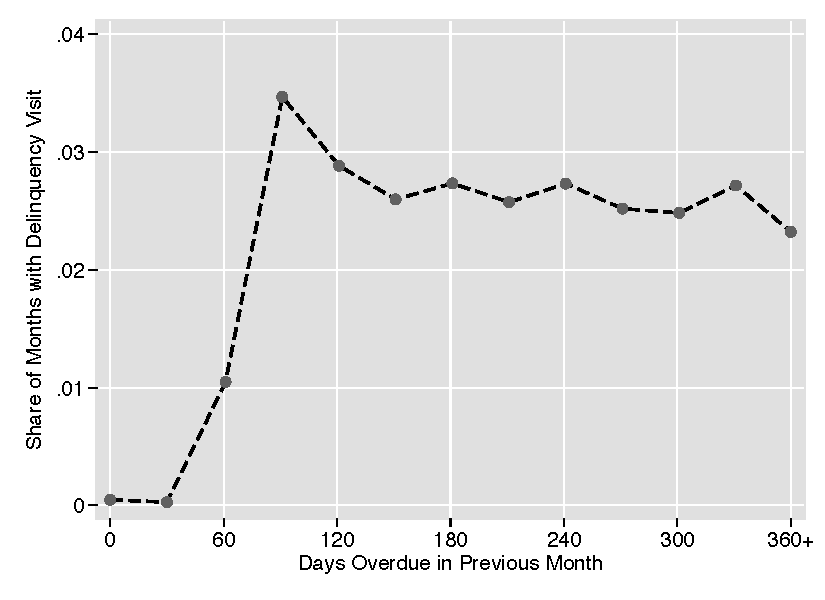
\includegraphics[scale=.7]{tables/connected_visit_hazard_all.pdf}
\end{figure}

\begin{table}[h!]
\centering
\caption{Mean Characteristics by Delinquency Visit Status}\label{table:descriptives_3g}
\vspace{-2mm}
\begin{tabular}{l*{1}{ccc}}
\toprule
 & Never Visited & Stayers & Leavers  \\
% &   &         &        \\
\midrule
 Usage (m3)  & 24.3  & 26.2  & 26.3  \\ 
 Bill  & 658  & 761  & 833  \\ 
 Unpaid Balance  & 706  & 2,416  & 6,520  \\ 
 Share of Months with Payment  & 0.78  & 0.60  & 0.38  \\ 
 Payment Size  & 829  & 1,214  & 1,247  \\ 
 Days Delinquent  & 18.9  & 84.9  & 236.5  \\ 
 Delinquency Visits per HH  & 0.00  & 1.32  & 1.42  \\ 
 Months Disconnected  & 0.01  & 0.03  & 0.31  \\ 
 HH Size  & 5.2  & 5.6  & 5.7  \\ 
 Age of HoH  & 47.4  & 44.8  & 45.8  \\ 
 Low Skilled HoH  & 0.14  & 0.17  & 0.19  \\ 
 &  &  &  \\ 
 Total Households   & 23,727  & 8,260  & 2,419  \\ 
 Total Observations  & 1,464,945  & 509,959  & 148,431  \\ 

\bottomrule
\multicolumn{4}{l}{\scriptsize ``Never Visited'' includes HHs that never receive a delinquency visit.}\\  [-.5em]
\multicolumn{4}{l}{\scriptsize ``Stayers'' includes HHs with $\geq$1 visit and are connected for the last 6 months.}\\ [-.5em]
\multicolumn{4}{l}{\scriptsize ``Leavers'' includes HHs with $\geq$1 visit and are disconnected for $\geq$1 of the last 6 months.}\\ [-.5em]
\multicolumn{4}{l}{\scriptsize Bill, Unpaid Balance, and Payment Size are in PhP/month.} 
\end{tabular}
\end{table}

Table~\ref{table:descriptives_3g} provides mean characteristics according to whether and how households respond to delinquency visits over the course of the sample.  The first column, ``Never Visited,'' includes households that never receive a delinquency visit.  Since delinquency visits are relatively rare, the majority of observations fall into this category.  The second and third columns include households that receive at least one delinquency visit.   The second column, ``Stayers,'' also requires that households are connected for the final 6 months of the sample while the third column, ``Leavers,'' includes households that are disconnected for at least one of the final 6 months of the sample.  

Leavers are predominantly composed of households that permanently disconnect over the sample period, which likely occurs when households move out of their current residences.  These households often leave large outstanding balances that are almost never repaid due to difficulties tracking households across locations.  Frequent delinquency visits allow the utility to minimize this lost revenue.  % incentivize households to regularly pay and By incentivizing households to pay, 

Stayers include households that remain connected at the end of the sample despite receiving at least one delinquency visit over the duration.\footnote{Stayers also exclude 67households that the utility has flagged as ``permanently disconnected.''}  Compared to households that are never visited, stayers have much higher outstanding balances and days delinquent.  Their payments also occur less frequently but have larger average sizes.  Stayers spend 3\% of the sample period disconnected from service.  While temporarily disconnected, these households likely substitute to alternative water sources including sharing with neighbors, using from deepwells, or purchasing from local water vendors.\footnote{Table~\ref{table:descriptives_3g} indicates that even for households that are never visited, they remain disconnected during 1\% of months.  These disconnections include (1) households that receive a delinquency visit before the start of the sample (but later reconnected) and (2) households that notify the utility about their moving plans in advance and therefore, do not receive a delinquency visit before disconnecting.}  Stayers also have slightly larger household sizes, younger heads of household, and greater incidence of low-skilled employment than never visited households.  These demographic patterns are consistent with lower-income households having greater difficulty paying their bills on time.


\begin{figure*}[hbtp]
    \centering
    \vspace{2mm}
    \begin{subfigure}[b]{0.49\textwidth}
        \centering
        \caption[]{\small Share Disconnected}  
        \vspace{-1mm}
        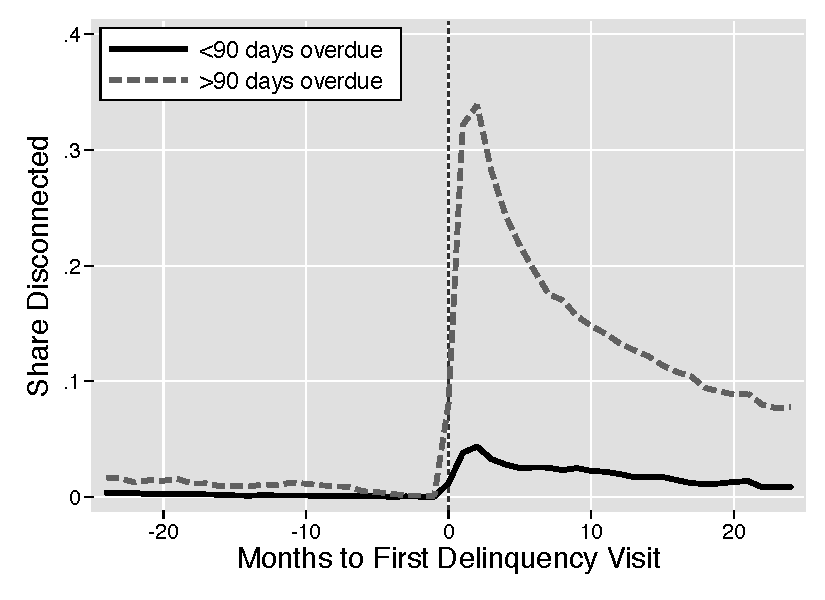
\includegraphics[width=\textwidth,trim={.2cm .2cm .2cm 0cm}, clip=true]{tables/line_disconnection}
        \label{fig:line_disc}
    \end{subfigure}
    \hfill
    \begin{subfigure}[b]{0.49\textwidth}  
        \centering 
        \caption[]{\small Unpaid Balance}
        \vspace{-1mm}
        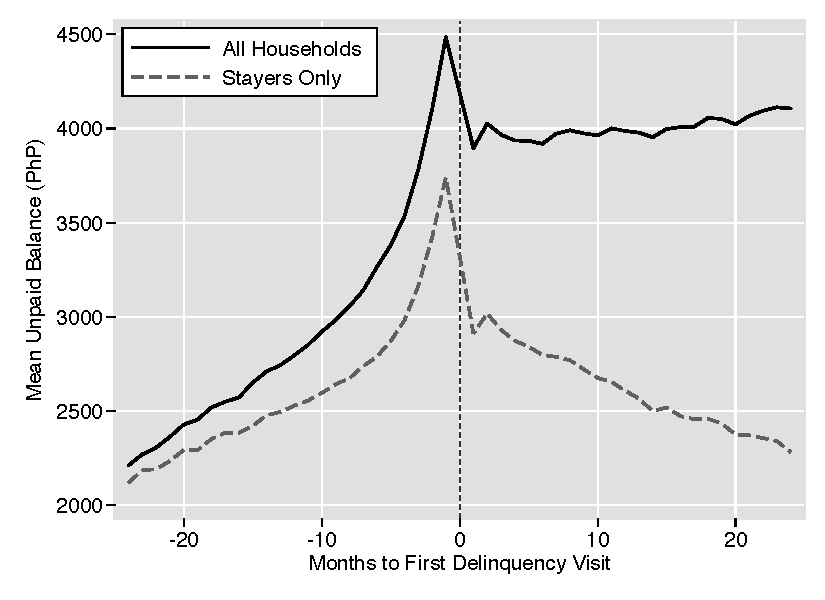
\includegraphics[width=\textwidth,trim={.2cm .2cm .2cm 0cm}, clip=true]{tables/line_bal}
        \label{fig:line_bal}
    \end{subfigure}
    \vskip 1mm \vskip 0pt
    \begin{subfigure}[b]{0.49\textwidth}
        \centering
        \caption[]{\small Days Overdue}
        \vspace{-1mm}
        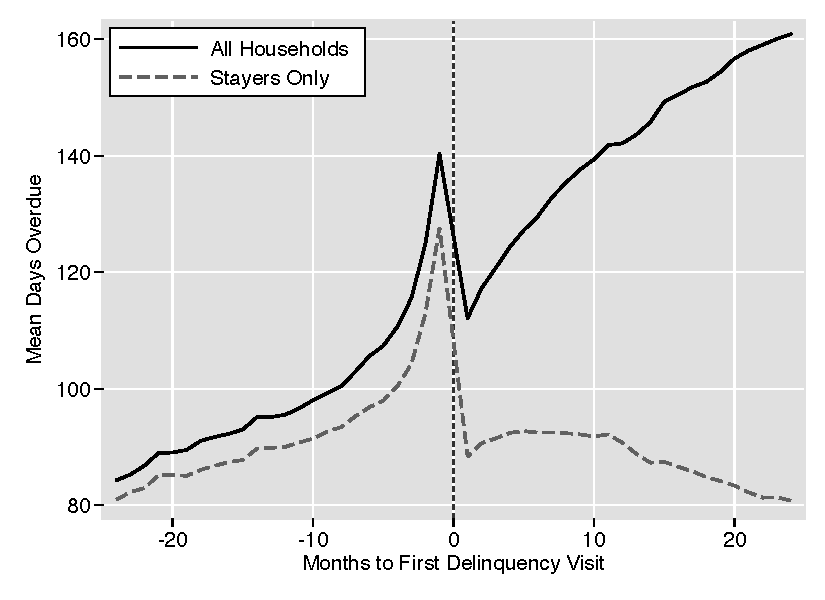
\includegraphics[width=\textwidth,trim={.2cm .2cm .2cm 0cm}, clip=true]{tables/line_ar}
        \label{fig:line_ar}
    \end{subfigure}
    \hfill
    \begin{subfigure}[b]{0.49\textwidth}  
        \centering
        \caption[]{\small Monthly Payment}  
        \vspace{-1mm}
        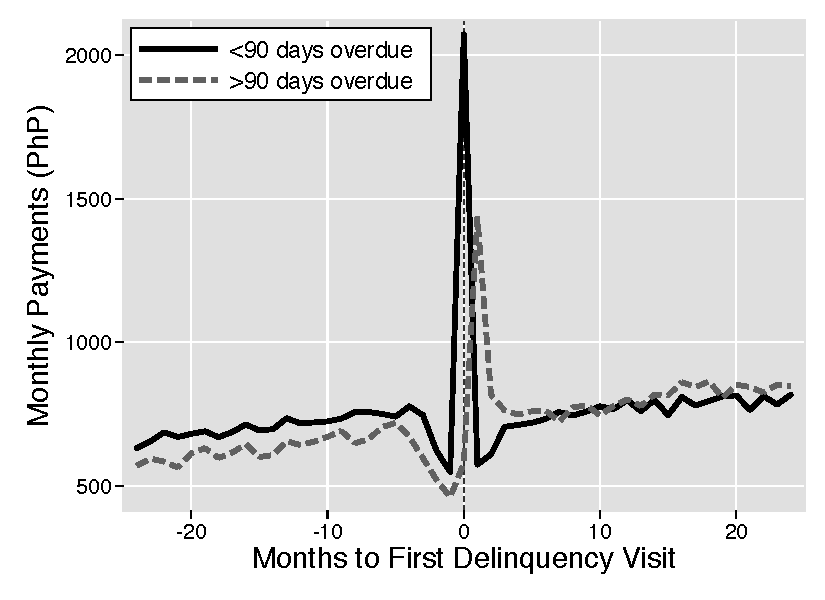
\includegraphics[width=\textwidth,trim={.2cm .2cm .2cm 0cm}, clip=true]{tables/line_pay}
        \label{fig:line_pay}
    \end{subfigure}
    \vskip 1mm \vskip 0pt
    \begin{subfigure}[b]{.49\textwidth}  
        \centering
        \caption[]{\small Average Consumption} 
        \vspace{-1mm}
        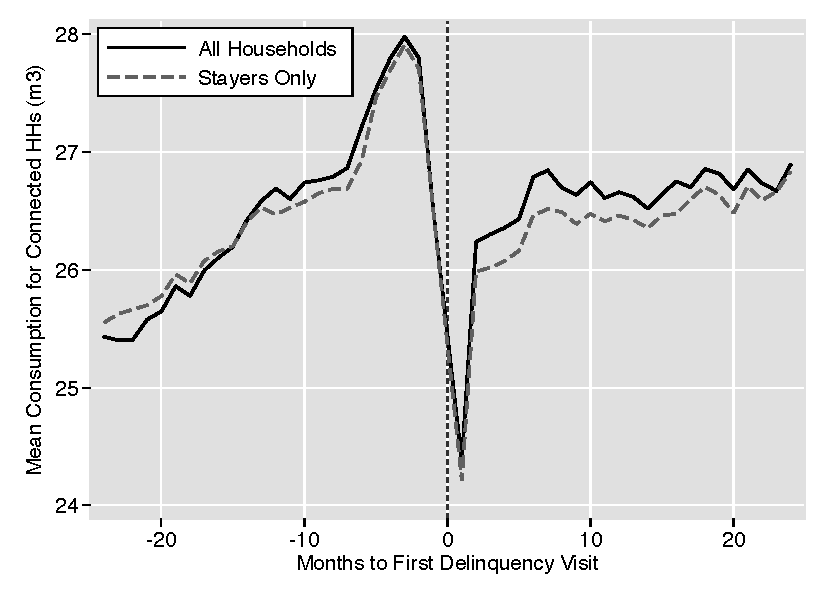
\includegraphics[width=\textwidth,trim={.2cm .2cm .2cm 0cm}, clip=true]{tables/line_c}  
        \label{fig:line_c}
    \end{subfigure}
    \hfill \hspace{.02\textwidth}
    \begin{minipage}{0.47\textwidth}   
    \vspace{-6cm}
    \caption[]
    {\small Mean Outcomes around First Delinquency Visit  \\  \\  Figures include all households with delinquency visits.  Stayers include only households who are connected for the last 6 months of the sample.  Mean monthly payments include zeros when no payment is made. } \label{fig:line_graphs}
    \end{minipage}
\end{figure*} 


To investigate how households respond to delinquency visits, Figure~\ref{fig:line_graphs} plots monthly mean outcomes in months relative to the first delinquency visit for each household.  Outcomes are plotted separately for all households that experience delinquency visits as well as for stayer households who experience visits and also remain connected for the last 6 months of the sample.  By definition, ``Never Visited'' households are excluded in Figure~\ref{fig:line_graphs}.  In the months just preceding a visit, monthly payments (Figure~\ref{fig:line_pay}) decrease suddenly, leading to corresponding increases in unpaid balances (Figure~\ref{fig:line_bal}) and days overdue (Figure~\ref{fig:line_ar}).  Average consumption (Figure~\ref{fig:line_c}) increases slightly as well.  In these months, stayers follow similar patterns but with lower levels of delinquency than the population average.

Immediately following the first delinquency visit, monthly payments spike as many households pay their full outstanding balances to prevent any disconnection.  Despite these payments, the average share of households disconnected (Figure~\ref{fig:line_disc}) also spikes to around 24\unskip\% before decreasing, as some households pay for reconnection, and stabilizing at 17\unskip\%, which is likely composed of households who have chosen to permanently disconnect from service.  Compared to the population average, stayer households pay more and disconnect less just following a visit.  Disconnection rates for stayers spike to 15\unskip\% before declining to 4\unskip\% around two years later.\footnote{Although stayers are connected for the last 6 months of the sample by definition, disconnection rates do not decline to zero since some stayers experience multiple temporary disconnection spells.}  The decline among stayers accounts for much of the average decline in disconnection rates across the sample.  Although many stayers quickly reconnect within 6 months, reconnections continue accumulating beyond one year after a visit.  

This descriptive evidence indicates that many households choose to disconnect for long periods before finally paying for reconnection.  This behavior is consistent with households facing credit-constraints, which prevent them from taking a low-cost loan to fund immediate reconnection.  Instead, households may substitute to lower-quality alternative sources of water until they can save enough income for reconnection.  Credit constraints would additionally predict that the most delinquent households at the time of the visit may be the most likely to disconnect following a visit.  The data support this hypothesis, finding that the share disconnected two months after a visit is 32\unskip\% for stayers that are over 90 days delinquent at the time of the visit.  The corresponding share for stayers under 90 days delinquent shrinks to 4\unskip\%.

Another hypothesis may be that households choose to stop paying when they leave their homes for vacation or overseas work.  This mechanism would likely predict a large decrease in water consumption in the months preceding delinquency visits.  Instead, consumption rises consistently between 24 and 2 months before a visit.\footnote{By contrast, Appendix~\ref{appendix:permanentdc} plots consumption relative to permanent disconnections and finds larger increases in water consumption just prior to permanently disconnecting.}  This consumption rise is consistent with households substituting toward water consumption in months where they are credit constrained.  Consumption then drops one month before, during, and after a visit, before quickly returning to an average level.  This dip in consumption likely corresponds to connections that are disconnected for less than a month before being reconnected and having their consumption recorded for that month.  Overall, this variation is relatively small given a mean consumption for stayers of 26.7m3 with a standard deviation of 11.1\unskip.  Moreover, delinquency visits are relatively rare, which may make their exact timing difficult for households to predict.  











%The administrative data indicate that 72.5\unskip\% resolve their outstanding balances following a notice.

% At this time, households report paying 

%In practice, the water company often tolerates delinquency well over 60 days, which is consistent with (1) costs of sending and following up on notifications and (2) household demand for credit from the water company.  Households receive notice in 0.66\unskip\% of months.  

% This rate increases to 1.75\unskip\% for households with at least 60 days of delinquency.  

% Figure~\ref{figure:dc_hazard} graphs the probability of receiving a delinquency notice conditional on the level of delinquency for each account.  The water company appears to carefully follow government regulations preventing any disconnection for delinquency below 60 days.  Once households reach 61 days of delinquency, they face some probability of receiving a notice, which triples moving above 90 days unpaid balance.  Conditional on having greater than 90 days of delinquency 

%  In practice, the water company tolerates 108.1days of delinquency on average before issuing a notice.  The level of delinquency tolerated before issuing notices also appears uncorrelated with (list measures/demographics...).  ( SHOW REGRESSION IN APPENDIX )  

% Upon receiving a notice of disconnection, connection owners then negotiate for time to pay their outstanding balances.  In 96\unskip\% of notices, owners are agree to pay within 30 days, making an average grace period of 13days according to the water connection survey.  25\unskip\% of connections report having ``enough time'' to make their payments.  

% %The administrative data indicate that 72.5\unskip\% resolve their outstanding balances following a notice.

% Disconnection typically involves workers from the water company placing a metal lock on the water meter stopping the flow.  Once disconnected, connection owners are charged a small, one-time fee of 200 PhP to restore their water service on top of settling any outstanding balances.  The water company is then required to restore service within 48 hours of receiving full payment for reconnection.

% \begin{itemize}
% \item No notice: great access to credit, or just not enough time to observe them hitting a
% \item Average notice rate!?!
% \end{itemize}
%\footnote{To account for potential mismeasurement in the administrative data, this measure allows connection owners to resolve their outstanding balances within 60 days of receiving notice.}
% In practice, .\unskip\% of owners report receiving advanced notice.  

\section{A Model of Borrowing, Saving, and Water Use}\label{section:model}

%\subsection{Setting up the Household's Problem}
%Time horizon etc.  Ignore disconnecting households.. 


To model household borrowing and decisions saving alongside water demand, I start from a standard intertemporal utility maximization problem as developed by \cite{deaton1991saving}.  This approach assumes an infinite time horizon where households choose water usage, borrowing, and savings in each period to maximize current and expected future utility.  Household expected utility is given by the following equation
\begin{align}\label{eq:u}
E_t \Big[ \sum_{\tau = t}^{\infty} (1+\delta)^{t-\tau} u(w_{\tau},x_{\tau})   \Big]
\end{align}
where utility in each period $t$ is expressed as an increasing and concave function of water usage, $w_{t}$, and consumption of all other goods, which are collapsed into a single bundle, $x_{t}$.  Households have a rate of time preference $\delta \in (0,1)$.  In each period, households face a budget constraint as follows
\begin{align}\label{eq:bc}
x_t \, + \, p(w_t) w_t \, &= \, y_t \, - D_{t+1} f  \, + \, S_t \, - \, S_{t+1}
\end{align}
where $p(w_t)$ captures the price per unit of water and may fluctuate with water use according to the water tariff structure.\footnote{For example, Manila has a steeply increasing price schedule with monthly usage, which is described in more detail in Appendix~\ref{appendix:tariff}.}  The price of other goods, $x_t$, is normalized to one.  $y_t$ represents household income each period which takes a value of $(1+\theta)\bar{y}$ with probability $\pi \in (0,1)$ and a value of $(1-\theta)\bar{y}$ with probability $(1-\pi)$ where $\theta  \in (0,1)$.  At the beginning of each period, households can choose whether to be temporarily disconnected ($D_{t+1}=1$) or connected ($D_{t+1}=0$) to water service.  If households disconnect (or remain disconnected), they pay a fixed cost $f$.  Since temporarily disconnected households are likely to share with neighbors or purchase from local vendors who resell piped water, they are assumed to face the same price per unit, $p(w_t)$, as connected households.  Temporary disconnection allows households to delay paying their outstanding water balances, especially after receiving a delinquency visit, as described in more detail below.  

By delaying payment of water bills, households are able to borrow against their future income realizations.  $S_t$ captures total assets chosen in the previous period to be consumed in period $t$ while $S_{t+1}$ captures total assets set aside in period $t$ for consumption in $t+1$ %Total assets in each period can be expressed in terms of two types, $A_t$ and $B_t$ given by the following expression
\begin{align}
S_t &= A_t + B_t \\
S_{t+1} &=  \dfrac{A_{t+1}}{1+r^{a}_{t}}  + I_t \dfrac{B_{t+1}}{1+r^{b}_{t}} 
\end{align}
$A_t$ captures standard assets for borrowing and saving.  The real interest rate $r_a$ is assumed to take a value of $r_l$ when households are saving ($A_{t+1} \leq 0$) and a value of $r_h$ when households are borrowing ($A_{t+1} > 0$).  This wedge in interest rates is intended to capture an institutional context with underdeveloped financial markets where households face high borrowing costs from moneylenders as well as high transaction costs in loaning out their own savings.  This assumption is consistent with a recent literature in development economics that emphasizes how households often savings and borrowing constraints.\footnote{In Kenya, \cite{dupas2013savings} and \cite{dupas2013don} estimate large willingness-to-pay for improved savings technologies.  In Manila, \cite{karlan2009expanding} find high  interest rates for loans from moneylenders.}  Households are assumed to be unconstrained in their amount of borrowing or saving with this asset.  % possibly cite (\cite{karlan2009expanding}) here?

$B_t$ captures borrowing through unpaid water bills.  Households face a real interest rate $r_b$ for borrowing from water bills.  To prevent arbitrage cases where households borrow infinitely from water bills to invest in standard assets, $r_b$ is assumed to equal $r_h$ when households are saving through standard assets ($A_t>0$), and is equal to $r_w$ otherwise.  $r_w$ is equal to zero in the context of Manila since the utility is not allowed to charge interest on outstanding balances.%This assumption is also consistent with some transaction costs in switching between asset types.
% and $D_{t+1}$ is an indicator for the household's disconnection choice given their disconnection status inherited from the previous period, $D_t$

$I_t$ is an indicator that determines when households are able to borrow from their unpaid water bills and takes the following form
\begin{align}
I_t = D_{t+1} + (1-c_t) (1-D_t) (1-D_{t+1})
\end{align} %I_t = (D_{t+1} + c_t (1-D_{t+1})(1-D_t)) 
where $c_t$ is an indicator for whether a household receives a delinquency visit, which occurs with probability $\lambda \in (0,1)$ in each period.  If households receive a delinquency visit ($c_t=1$) and they choose to remain connected ($D_{t+1}=0$), then they must pay their full outstanding balance to remain connected, which means that households cannot continue borrowing against their unpaid water bill this period meaning that $I_t=0$.  Similarly, if currently disconnected households ($D_t=1$) want to reconnect ($D_{t+1}=0$), then they also need to pay their full outstanding balance this period meaning that $I_t=0$.  Choosing to disconnect ($D_{t+1}=1$) allows households to avoid paying their unpaid balances until they choose to reconnect, meaning that $I_t=0$ in the current period.  

Given that households are able to borrow, the amount that they can borrow through unpaid bills is constrained as follows
\begin{align}\label{eq:borrowconstraint}
&B_t -  p(w_t) w_t (1-D_{t+1})(1+r_b) \leq B_{t+1} \leq 0 
\end{align}
By leaving bills unpaid, households are able to borrow up to their outstanding balance inherited from last period, $B_t$, plus their total bill from water consumption this period, $p(w_t) w_t$, given that they remain connected to water service ($D_{t+1}=0$).  If households choose to disconnect ($D_{t+1}=1$), then they can keep borrowing up to their existing outstanding balance, $B_t$, but they cannot add to this balance through unpaid water use.  To capture the empirical fact that water bills are almost never overpaid, households are assumed to be unable to save with this asset.

This framework results in four possible states depending on whether income, $y_t$, is high or low and whether households receive a delinquency visit given by the indicator variable, $c_t$.  Assuming that the probabilities of reaching each state are uncorrelated with each other yields the following transition matrix between states

% \resizebox{.73\linewidth}{!}{
%   \begin{minipage}{\linewidth}
% \begin{align}
% \begin{split}
% \label{eq:tmatrix}
% T_{t,t+1} &= \bordermatrix{\text{} & y_t=(1+\theta)\bar{y}\,,\,c_t=0 & y_t=(1-\theta)\bar{y}\,,\, c_t=0 & y_t=(1+\theta)\bar{y}\,,\,c_t=1 & y_t=(1-\theta)\bar{y}\,,\,c_t=1 \cr
%                 y_t=(1+\theta)\bar{y}\,,\, c_t=0 & \pi (1-\lambda) & (1-\pi) (1-\lambda) & \pi \lambda & (1-\pi) \lambda  \cr
%                 y_t=(1-\theta)\bar{y}\,,\, c_t=0 & \pi (1-\lambda) & (1-\pi) (1-\lambda) & \pi \lambda & (1-\pi) \lambda  \cr
%                 y_t=(1+\theta)\bar{y}\,,\, c_t=1    & \pi (1-\lambda) & (1-\pi) (1-\lambda) & \pi \lambda & (1-\pi) \lambda  \cr
%                 y_t=(1-\theta)\bar{y}\,,\, c_t=1  & \pi (1-\lambda) & (1-\pi) (1-\lambda) & \pi \lambda &  (1-\pi) \lambda  }
% \end{split}
% \end{align}
%   \end{minipage}
% }

\resizebox{.85\linewidth}{!}{
  \begin{minipage}{\linewidth}
\begin{align}
\begin{split}
\label{eq:tmatrix}
T_{t,t+1} &= \bordermatrix{\text{} & (1+\theta)\bar{y}\,,\,\text{no visit} & (1-\theta)\bar{y}\,,\,\text{no visit} & (1+\theta)\bar{y}\,,\,\text{visit} & (1-\theta)\bar{y}\,,\,\text{visit} \cr
                (1+\theta)\bar{y}\,,\,\text{no visit} & \pi (1-\lambda) & (1-\pi) (1-\lambda) & \pi \lambda & (1-\pi) \lambda  \cr
                (1-\theta)\bar{y}\,,\,\text{no visit} & \pi (1-\lambda) & (1-\pi) (1-\lambda) & \pi \lambda & (1-\pi) \lambda  \cr
                (1+\theta)\bar{y}\,,\,\text{visit}    & \pi (1-\lambda) & (1-\pi) (1-\lambda) & \pi \lambda & (1-\pi) \lambda  \cr
                (1-\theta)\bar{y}\,,\,\text{visit}  & \pi (1-\lambda) & (1-\pi) (1-\lambda) & \pi \lambda &  (1-\pi) \lambda  }
\end{split}
\end{align}
  \end{minipage}
}

%\subsection{Solving the Model}

Given these definitions, the household's problem can be reformulated using a recursive value function approach where the household solves for a function, $V(X_t,z_t)$, that maximizes both current utility and the expected continuation value given the household's current asset-levels and their disconnection status, which are captured by $X_t$, as well as the current state given by $z_t$ in the following problem
\begin{align}\label{eq:valmax}
\begin{split}
V(X_t,z_t) \,=\, &max_{x_t,w_t}  \,\,\, u(x_t,w_t) \,+\,\, (1+\delta)^{-1} \, E \Big[\, V(X_{t+1}|z_{t})\,\Big| z_{t+1}, T_{t,t+1} \Big]
\\
s.t.& \\
x_t & \, + \, p(w_t) w_t \, = \, y_t \, - D_{t+1} f  \, + \, S_t \, - \, S_{t+1} \\
-p&(w_t) w_t (1-D_{t+1}) \leq \frac{B_{t+1}-B_t}{(1+r_b)} \leq 0  \\
X_t &= [A_{t},B_{t},D_{t}] \\
z_t &= [y_t,c_t]
\end{split} 
\end{align}
This problem can be solved in two steps: (1) maximizing utility within a given period by choosing $w_t$ and $x_t$ holding assets fixed, and (2) choosing assets to maximize utility over time.

% household's targeted amount of borrowing through unpaid water bills exceeds the amount of water that they would % except in cases where they need to overconsume water to raise enough revenue through unpaid water bills to meet their borrowing goals. 
Within each period, households solve a standard utility maximization problem over water, $w_t$, and other goods, $x_t$, subject to a budget constraint determined by their current income as well as current and future assets, which are taken as given for this step.  When given asset levels require borrowing through unpaid water bills, households face an additional constraint: they need to consume enough water this period to fund their water borrowing target.  For example, households may drink tap water instead of soft drinks or other beverages in months where they are especially credit constrained.  Formally, this situation occurs when equation (\ref{eq:borrowconstraint}) is binding.  

To express these constraints formally, let $L = \frac{B_{t+1} - B_t }{1+r^{b}_{t}}$ indicate the amount of revenue needed to be raised through water consumption to fund given borrowing targets.  Likewise, let $Y = y_t  - D_{t+1} f   +  A_t + B_t  -  \frac{A_{t+1}}{1+r^{a}_{t}} - I_t \frac{B_t}{1+r^{b}_{t}}$ equal all other net income used for consumption this period.  Also, let utility take a Cobb-Douglas shape in water and all other goods with preference parameter, $\alpha \in (0,1)$.  Cobb-Douglas preferences assume that households spend a constant share of their income on water and that the price-elasticity of demand for water is equal to one, which is in range with recent estimates in the literature.\footnote{\cite{wjv} finds an average price elasticity of 0.84 in this setting while \cite{szabo2015value} finds an average price elasticity of 0.98 in South Africa.  Other studies find elasticities ranging from 0.01 to 0.81 (\cite{diakite2009proposal}, \cite{strand2005water}).}  The Cobb-Douglas utility function is also assumed to take a log-log form, which assumes that households have a moderate demand for smoothing income over time.  Appendix~\ref{appendix:utilityshape} discusses this assumption in more detail.

The price of water is parameterized as a linear function of water use, $p(w) = p_1 + p_2 \, w$, to approximate the increasing block tariff present in Manila.  Suppressing most time subscripts for ease of exposition, the household maximization problem takes the following form within each period
\begin{align}\label{eq:hhmax}
\begin{split}
&max_{w_t,x_t} \,\,\,\, \alpha\, log(w) \, + \, (1-\alpha)\,log(x) \\
s.t.& \\
\,\,\,\, &(p_1 + p_2 w)\,w + x  =  Y - L \\
&(p_1 + p_2 w)\,w (1-D_{t+1}) \leq L  
\end{split}
\end{align}
Optimal consumption takes a piecewise form depending on whether households have to increase their water use to satisfy their demand for borrowing
\begin{align}\label{eq:ws}
\begin{split}
w^{*} &= 
\begin{cases}
                                                                                                                                                                                                                                                                                                                                                             \frac{p_{1}-\sqrt{{p_{1}}^2-8\,L\,\alpha \,p_{2}+8\,Y\,\alpha \,p_{2}+4\,L\,\alpha ^2\,p_{2}-4\,Y\,\alpha ^2\,p_{2}}}{2\,p_{2}\,\left(\alpha -2\right)}
 &\text{ if } L \geq \widehat{L} \\
                                                                                                                                                                                                                                                                                                                                                                                                                                                                -\frac{p_{1}-\sqrt{{p_{1}}^2-4\,L\,p_{2}}}{2\,p_{2}}
 &\text{ if } L < \widehat{L}
\end{cases} \\
&\widehat{L} =                                                                                                                                                                                                                                                                                                                                 \frac{Y}{2\,\left(\alpha -1\right)}+\frac{\frac{Y\,p_{2}}{2}+\frac{{p_{1}}^2}{8}-\frac{p_{1}\,\sqrt{{p_{1}}^2-\alpha \,{p_{1}}^2+8\,Y\,\alpha \,p_{2}}}{8\,\sqrt{1-\alpha }}}{p_{2}}

\end{split}
\end{align}
where $\widehat{L}$ captures the point at which revenue demanded for borrowing is exactly generated by the household's optimal consumption.  When borrowing demand outpaces revenue from optimal consumption (ie. $L<\widehat{L}$), then households must deviate from their optimal unconstrained consumption choice and instead consume enough water to exactly satisfy borrowing demand.\footnote{Note that a greater negative $L$ signals more borrowing.}  This overconsumption captures a potentially important inefficiency associated with using unpaid water bills as a source of credit.  Combining optimal consumption in equation (\ref{eq:ws}) with the budget constraint in equation (\ref{eq:bc}) as well as the utility function in equation (\ref{eq:hhmax}) results in an indirect utility function as a function of prices, income, and assets.  The full indirect utility function is given by equation (\ref{eq:vstar}) in Appendix~\ref{appendix:indirectutil}.

Given indirect utility in each period and a discount rate that is assumed to be greater than the return on savings (so that households do not save infinitely), $\delta> r_l$, households solve for a stationary value function in (\ref{eq:valmax}) that maximizes utility by mapping any combination of asset levels in period $t$ into optimal future asset levels in period $t+1$.

\section{Estimation and Results}\label{section:estimation}    % https://www.cgdev.org/blog/compartamos-context

The goal of the estimation strategy is to map variation in payment behavior, temporary disconnections, and monthly consumption into estimates of income variation, borrowing costs, and preferences for water.  Since identification relies heavily on the household's behaviors in response to delinquency visits, the estimation sample is limited to ``stayers'' --- households that experience delinquency visits but remain connected for the last six months of the sample as described in Section~\ref{section:descriptives}.  Table~\ref{table:descriptives_stayers} of Appendix~\ref{appendix:stayerdescriptives} includes detailed descriptive statistics for stayer households and Figure~\ref{figure:dc_hazardstayers} provides the probability of receiving a delinquency visit conditional on the days delinquent in the previous month for stayers.  Focusing on stayers may limit the generalizability of the results, especially given that stayers somewhat differ demographically from the population of households as shown in Table~\ref{table:descriptives_3g}.

Table~\ref{table:calibratedparam} describes parameters that are assumed or calibrated prior to estimation.  The monthly savings interest rate is calibrated to the prevailing interest rate in the Philippines over this time period.  The estimation assumes a monthly discount rate of 2\%, which implies an annual discount rate of 26.8\% and falls in the range of recent structural and experimental estimates.\footnote{\cite{andreoni2012estimating} estimate rates between 25\% and 35\% in an experimental setting and confirm exponential discounting.  \cite{laibson2007estimating} use a similar consumption-savings structural approach and recover a discount rate of around 15\%.  \cite{gourinchas2002consumption} use a similar structural approach finding a lower discount rate of around 5\%.}  Since this discount rate is assumed to exceed the savings interest rate, households are able to solve for a well-defined value function.

To measure prices, the non-linear tariff structure is approximated by a linear function of monthly usage as described in more detail in Appendix~\ref{appendix:tariff}.  This simplification allows for computational tractability within the dynamic model.\footnote{\cite{wjv} and \cite{szabo2015value} carefully capture non-linear pricing incentives with static models, which are very computationally expensive.}  This approach also parallels average pricing models of consumer demand for utilities as suggested by \cite{ito2014consumers}.  

Without monthly household income data, the estimation includes average income in Manila as measured by the 2015 Family Income and Expenditure Survey.  This method may overestimate true average household income because the estimation excludes shared water connections, which tend to used by poorer households.  At the same time, this approximation may underestimate true household income to the extent that the Family Income and Expenditure Survey includes households that are unconnected to piped water and also tend to be significantly poorer.\footnote{The 2010 Census of Population and Housing finds around 4 to 5\% of households were unconnected to piped water (\cite{wjv}).}  Households are assumed to face equal probabilities of high and low income shocks in any particular month while the size of monthly income shocks are estimated.  The last term needed for estimation is the risk of receiving a delinquency visit each month.  The risk of delinquency visits is calculated for the sample of stayer households who are over 31 days delinquent on their bills. % The last term needed for estimation is the risk of receiving a delinquency visit each month, which is calculated for the sample of stayers.

\begin{table}[H]
\centering
\caption{Calibrated and Assumed Parameters}\label{table:calibratedparam}
\vspace{-2mm}
\resizebox{\columnwidth}{!}{%
\begin{tabular}{l*{1}{ccl}}
\toprule
%Parameter  &   &  Value & Source \\
%\midrule
Savings Interest Rate & $r_l$ & 9.5\unskip\%  & {\footnotesize Philippines data from World Bank Databank (2010-2015) } \\
Water Interest Rate & $r_w$ & 0\% & {\footnotesize The regulator prevents charging interest on unpaid bills} \\
Discount Rate & $\delta$ & 2\% & {\footnotesize Mean of structural estimates from 
$\text{literature}^{\dagger}$} \\
Tariff    & $(p_1 + p_2 w)$ & $(20.226 + 0.3w)$ & {\footnotesize Estimated price by water usage  (See Appendix~\ref{appendix:tariff} for details) } \\
Mean Inc. (PhP) & $\bar{y}$ & 31,910 & {\footnotesize Family Income Expenditure Survey (2015) for Manila} \\
High Inc. Risk& $\pi$ & 50\% & {\footnotesize Assumed to ensure symmetric income shocks} \\
Visit Risk & $\lambda$ & 2.6\unskip\% & {\footnotesize \% of months with a visit among stayers with $>$31 days overdue} \\
\bottomrule
\multicolumn{4}{l}{\scriptsize All measures are monthly.  Annual rates are converted to monthly rates as follows: Monthly Rate = $(1+\text{Annual Rate})^{1/12}-1$} \\[-.5em]
\multicolumn{4}{l}{\scriptsize $\text{}^{\dagger}$ See \cite{andreoni2012estimating}, \cite{laibson2007estimating}, and \cite{gourinchas2002consumption} for structural $\delta$ estimates.}
\end{tabular}
}
\end{table}

  % M = (1 + A)^(1/12) - 1 % A = (1 + M)^12 - 1

Given assumed and calibrated parameters from Table~\ref{table:calibratedparam}, the estimation strategy is able to recover parameters described in Table~\ref{table:estimparam} using moments in the data.  Due to computational limitations, the estimation recovers a single set of parameters that apply to a representative household, which limits the generalizability of the results to particular subpopulations.  

Average consumption primarily identifies household water preferences.  With Cobb-Douglas preferences, identification rests on the assumption that household price elasticity is equal to one so that the preference parameter, $\alpha$, can be recovered mainly from the share of the household budget used on water.

Without data on monthly household income variation, the estimation strategy is designed to recover the magnitude of monthly income variation that rationalizes the amount of unpaid water bills observed in the data.  Under the structure of the model, greater income variation increases household demand for credit, which in turn increases the amount of unpaid water bills.  This approach assumes that the only reason that households choose not to pay their water bills is to smooth their consumption over time.  This assumption may not be valid in cases where households pay their bills infrequently because they face travel or other hassle costs in making each payment.  As discussed in Section~\ref{section:descriptives}, households have a variety of payment options available to them including through local convenience stores, online, and over the phone, which suggests that any additional costs of making each payment may be small. % ARE COMPLAINTS ALSO ZERO!?

The fixed cost of disconnecting and using from an alternative water source is recovered from the share of households that disconnect in response to a delinquency visit.  Disconnecting allows households to avoid immediately paying their outstanding water balances.  Therefore, high disconnection rates suggest low fixed costs of being disconnected.

The borrowing rate from standard assets is identified from differential disconnections rates in response to delinquency visits for households above and below 90 days overdue at the time of a visit.  This identification strategy leverages the intuition that many households with large debts at the time of a visit would require large loans in order to remain connected.  Therefore, high interest rates on these loans may especially drive these households to temporarily disconnect in response to a visit.  This identification strategy requires the assumption that households above and below 90 days overdue at the time of a visit face equal fixed costs of remaining disconnected.  For example, if more delinquent households have better outside options for water, then this approach would wrongfully attribute their high disconnection rates to high borrowing costs.  Also for this approach to be valid, households must be unable to predict the exact timing of delinquency visits.  While Appendix~\ref{table:tcd_predict} provides some evidence that the timing of delinquency visits is correlated with demographics and payment behavior, delinquency visits are relatively rare events and only 36\unskip\% of disconnected households reported receiving advanced warning from the utility.
%\footnote{TEST THE ASSUMPTION THAT OUTSIDE OPTIONS ARE THE SAME PLEASE?!}

\begin{table}[H]
\centering
\caption{Parameters to be Estimated}\label{table:estimparam}
\vspace{-2mm}
%\resizebox{\columnwidth}{!}{%
\begin{tabular}{l*{1}{cl}}
\toprule
Parameters  &   & Main Identifying Moments  \\
\midrule
Water Preference  & $\alpha$ & Mean Usage \\[.1em]
Income Shock Magnitude & $\theta$ & Mean Outstanding Balance  \\[.1em]
Fixed Cost of being Disconnected  & $f$ &  \% Disconnected 1-4 months post visit \\[.1em]
Borrowing Rate from Standard Assets & $r_h$ & \% Disconnected 1-4 months post visit \\
 & & given 90+ days overdue when visited \\
\bottomrule
%\multicolumn{3}{l}{\scriptsize All rates are monthly.  Annual rates are converted to monthly as follows: Monthly Rate = $(1+\text{Annual Rate})^{1/12}-1$} 
\end{tabular}
%}
\end{table}

The estimation routine solves the household's problem in equation (\ref{eq:valmax}) through value function iteration over a grid of asset values.  Households can choose from    10
values of the standard asset, $A_{t+1}$, evenly spaced across a mean zero normal distribution with a standard deviation of 10,000
\unskip, a minimum of -17,688
\unskip, and a maximum of 13,352
\unskip.  Households can also choose how much to borrow from unpaid water bills, $B_{t+1}$, over    11
values evenly spaced across a mean zero normal distribution truncated above at zero with a standard deviation of  3,800
and a minimum of -7,835
\unskip.  The additional choice of whether to stay connected each period, $D_{t+1}$, brings the total possible number of asset combinations to  1,300
\unskip.  

The estimation strategy uses a simulated method of moments approach, which chooses parameters to minimize the sum of squared distances between simulated and true moments, weighted by their average values in the data.  To generate simulated moments, the estimator creates a random  2,000
month chain of states according to the transition matrix (equation (\ref{eq:tmatrix})) and calculates the household's predicted asset and consumption choices across these states (assuming asset levels of zero to start).\footnote{See \cite{laibson2007estimating} and \cite{gourinchas2002consumption} for similar approaches to estimation.}

Table~\ref{table:estimates} provides the estimation results.  The Cobb-Douglas preference for water consumption is estimated to be 0.025
\unskip, which is consistent with households' observed budget share dedicated to water in Manila.  The estimated income shock of 0.342
implies that household income either increases or decreases by 20.7
\unskip\% of its average with 50\% probability each month.  This estimate can also be interpreted as measuring the coefficient of variation (CV) of income and falls on the lower end of previous estimates in the literature.\footnote{The coefficient of variation (CV) measures the standard deviation of monthly household income divided by average household income (\cite{hannagan2015income}).}  \cite{hannagan2015income} use monthly financial diaries in the US to calculate CVs of 0.39 for average households and 0.55 for households below the poverty line.  Using household surveys from Mexico, \cite{amuedo2011remittances} calculate CVs between 0.29 and 0.46. %, which more closely resemble the estimate in Table~\ref{table:estimates}

The estimation recovers a fixed cost of being disconnected of 198.9
PhP/month.  Previous research uses a static, structural approach to estimate a long-term monthly fixed cost from using alternative water sources of 130 PhP/month (\cite{wjv}).  While these estimates fall in a similar range, this paper produces a larger estimate of the fixed-cost likely because sudden disconnections leave little time for households to invest in finding low-cost alternative sources for water.  This estimate is also likely to capture the one-time 200 PhP fee charged to households for reconnection.

The borrowing rate from standard assets is estimated to be 2.2
\unskip\% per month, which implies an annual interest rate of 56.2
\unskip\%.  This estimate is substantially lower than the 20\% per month interest rate that \cite{karlan2009expanding} document as being commonly charged by moneylenders in Manila.  Despite this high interest rate, \cite{karlan2009expanding} document that at least 30\% of their sample of microentrepreneurs report taking credit from moneylenders.  The estimated borrowing rate of 2.2
\unskip\% is more similar to microloans of 1,000 PhP at 2.5\% monthly interest offered to rural Filipino households as part of a microfinance experiment conducted by \cite{gine2014group}.\footnote{The annual interest rate of 56.2
\unskip\% well exceeds the average 13 to 25\% range offered by microfinance providers worldwide surveyed by \cite{cull2009microfinance}.  Two possible reasons for this discrepancy are that (1) institutional reasons unique to Manila may limit lenders' abilities to offer low rates and (2) subsidies may allow many microfinance providers to offer below-market interest rates.}

\begin{table}[h!]
\centering
\caption{Estimates}\label{table:estimates}
\vspace{-2mm}
%\resizebox{\columnwidth}{!}{%
\begin{tabular}{l*{1}{cc}}
\toprule
Parameters  &   & Estimates \\
\midrule
Water Preference & $\alpha$ & 0.025
 \\
 &  & (0.00013
\unskip) \\[.4em]
Income Shock Magnitude & $\theta$ & 0.342
 \\
 &  & (0.0318
\unskip) \\[.4em]
Fixed Cost of being Disconnected (PhP) & $f$ &  198.9
 \\
 &  &  (0.0
\unskip) \\[.4em]
Borrowing Rate from Standard Assets & $r_h$ & 0.022
 \\
 &  & (0.0011
\unskip) \\[.8em]
Households & & 11,856 \\
Household-Months & & 731,935 \\
\bottomrule
\multicolumn{3}{l}{\scriptsize Standard errors in parentheses are bootstrapped at the household-level.} % with 4
repetitions 
\end{tabular}
%}
\end{table}

Table~\ref{table:fit} provides both moments in the data used for estimation as well as other moments to help understand the fit of the model.  While the model is able to almost exactly match average usage and outstanding balance, the model has more difficulty matching the slow decline in disconnection rates observed after delinquency visits.  The model instead predicts that households who disconnect in response to a delinquency visit will quickly reconnect over the following four months.  One explanation for this discrepancy may be that the distribution of income shocks does not allow for serial correlation so that households are assumed to quickly recover from negative shocks in the model.  In reality, households may be temporarily disconnecting in response to longer-term negative income shocks like job-loss or illness.  A similar pattern exists for disconnection conditional on being at least 90 days overdue when visited.

\begin{table}[H]
\centering
\caption{Model Fit}\label{table:fit}

\begin{tabular}{l*{1}{cc}}
\toprule
 Moments & Data  & Predicted \\[.5em]
Used in Estimation & & \\
\midrule
Mean Usage (m3) &26.20&26.20\\
Mean Water Debt (PhP) &2415.8&2341.1\\
[.5em]
\% Disconnected Post-Visit  & & \\[.2em]
1 month &0.13&0.12\\
2 months &0.14&0.10\\
3 months  &0.12&0.06\\
4 months &0.10&0.05\\[.8em]
\% Disconnected Post-Visit & & \\
given 90+ days overdue when visited & & \\[.2em]
1 month &0.30&0.28\\
2 months &0.32&0.23\\
3 months &0.26&0.13\\
4 months &0.23&0.11\\
& & \\
Unused in Estimation & & \\
\midrule
SD Usage &12.3&2.4\\
SD Outstanding Balance  &3588.7&2634.7\\
Corr. Usage and Out. Bal. &0.31&-0.02\\

\bottomrule
\multicolumn{3}{l}{\scriptsize ``SD'' stands for standard deviation and ``Corr.'' stands for correlation. }  \\[-.5em]
\multicolumn{3}{l}{\scriptsize ``Out. Bal.'' stands for outstanding balance. Standard deviations in the data }  \\[-.5em]
\multicolumn{3}{l}{\scriptsize are calculated with variation within households.}
\end{tabular}
%\begin{tabular}{lcc}
& Data & Estimated \\
Mean Usage (m3) &24.9&25.5\\
SD Usage &11.1&2.2\\
Mean Water Debt (PhP) &1232&1222\\
SD Water Debt (PhP) &1281&1821\\
Corr. Usage and Water Debt &0.34&-0.01\\
Mean Usage Pre-Collect (m3) &26.2&25.2\\
Mean Usage Post-Collect &23.4&22.7\\
Diff. (Pre-Post) (m3) &2.8&2.5\\
\end{tabular} 

\end{table}

The model has difficultly matching moments that were not used in the estimation.  Since log-utility encourages households to smooth their consumption over time, this model predicts very little variation in water usage over time.  By contrast, high observed variation in usage is likely driven by the fact that households face idiosyncratic shocks to their water demand each month as household members travel for work, other families come to visit, or Manila experiences a heat wave.  A more complete model may include a term for indiosyncratic water shocks although it is unclear whether these shocks would substantively affect the model's predictions for income smoothing across time.  While poorly matching variation in usage, the model is able to generate over half of the observed variation in outstanding balances.  

The data find a positive correlation between usage and outstanding balances, which suggests that households may take on water debt to fund extra consumption in months where they face large, positive shocks to their water demand.  In the model, positive income shocks reduce demand for water debt and increase demand for water. At the same time, negative income shocks reduce demand for water while increasing demand for water debt.  On net, the model finds zero average correlation between outstanding balances and usage. % Therefore, in some cases, households use more water during negative income shocks in order to increase their borrowing limits.     

\begin{figure}[H]
\centering
\caption{100 Months of Simulated Data around \\ a Period of Disconnection}\label{figure:deaton}
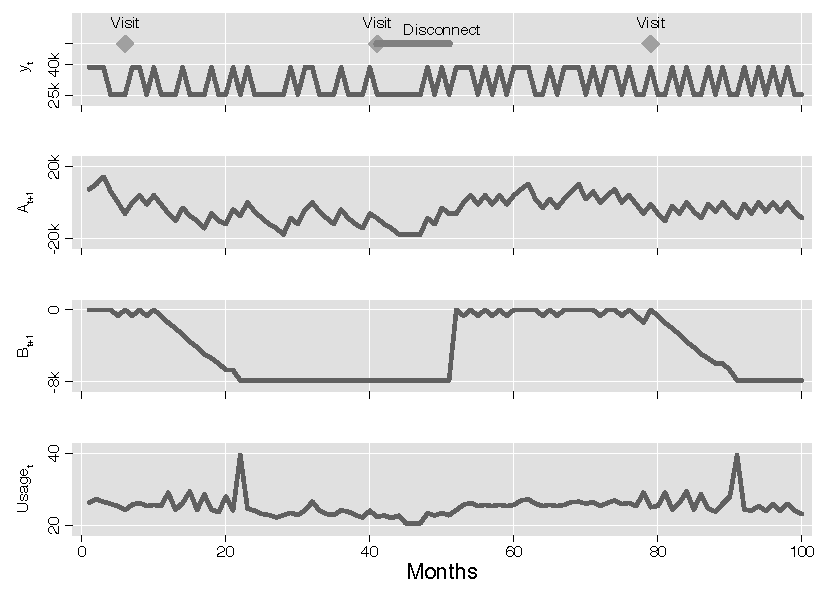
\includegraphics[scale=1.1]{tables/new_deaton_graph.pdf} \\
{\scriptsize  
Note: 100 months are chosen to center around the first disconnection event in the  2,000
month random sequence of income and delinquency visit states used in the estimation.  ``Visit'' indicates months with a delinquency visit with a diamond.  ``Disconnect'' indicates months disconnected with a thick line.  Cum. $\Delta y_t$ measures cumulative shocks to income in PhP, $A_{t+1}$ indicates the optimal position for standard assets in PhP, $B_{t+1}$ indicates the optimal amount of water borrowing in PhP, and $\text{Usage}_t$ indicates water consumption in m3.
\par}
\end{figure}


To build intuition, Figure~\ref{figure:deaton} provides 100 time periods of simulated data from the model.  These 100 time periods are chosen to center around the first disconnection occurrence in the  2,000
month random sequence of states used in the estimation.  The first panel in Figure~\ref{figure:deaton} indicates the cumulative, exogenous income shocks faced by the household.  This sample begins with a long period where negative income shocks occur more frequently than positive income shocks.  Positive shocks only begin to outweigh negative shocks at around 50 months.  Indicators for when the household receives delinquency visits as well as whether it chooses to remain disconnected are also nested in this first panel.  Over the course of 100 months, the household experiences three visits, the second of which leads the household to disconnect for around 12 months.  This disconnection corresponds to a period where the household has accumulated a long string of negative income shocks.

The second panel indicates the household's choice of asset position, $A_{t+1}$, in each month.  Asset position closely tracks income realizations as the household increasingly borrows (moving into very negative positions) following the long series of negative income shocks.  At around the time of disconnection, the household chooses to borrow the maximum allowed by the grid of assets chosen for the simulation.  Positive income shocks then allow the household to borrow less and begin saving at around 60 months.

The third panel indicates household borrowing through unpaid water bills, $B_{t+1}$.  In the beginning, the household increases its borrowing more slowly than with standard assets since each month's increase in borrowing is limited by the size of the household's current water bill.  Matching the downturn in income, the household continues borrowing before reaching the maximum borrowing allowed by the grid of assets chosen in this simulation.  With few positive income shocks, the household remains at this maximum borrowing level for at least 24 months.  When the second delinquency visit occurs at around 40 months, the household is still borrowing the maximum from unpaid water bills and therefore, instead of choosing to pay its full outstanding balance to stay connected, the household chooses to disconnect until it accumulates enough positive income shocks to pay its full water bill around month 55.  During the third delinquency visit, the household's outstanding balance happens to be relatively small so it is able to immediately pay in full to remain connected.

The fourth panel indicates household water usage patterns over the same 100 months.  Usage begins to spike as the household increases its usage to fund borrowing through unpaid water bills.  The largest spikes in usage occur when the household moves to the maximum level of borrowing.  Because of the step-size chosen for the asset grid, moving to the largest borrowing level requires a jump in unpaid bills of around 1,000 PhP.  Since the average bill is around 600 PhP, the household needs to almost double its usage to fund this jump in borrowing from unpaid bills.  These spikes in usage measure the extent to which borrowing from unpaid water bills may distort consumption choices, adding an additional friction associated with borrowing from water bills.  After maximizing water borrowing at around 24 months, usage begins to stabilize at lower levels, mirroring the long string of negative income shocks faced by the household.  Usage recovers to a higher level after the second delinquency visit before spiking again as the household maximizes its water debt in the last several months.

\section{Counterfactual Policies}\label{section:counterfactuals}
%In practice, this counterfactual setting may correspond to a policy of strict enforcement by the utility (ie. monthly delinquency visits). 
To measure how much households value credit from unpaid water bills, I examine how household welfare changes in a counterfactual setting where households are unable to borrow from their water bills.  Table~\ref{table:counter} includes outcomes for the current setting in Manila in Column (1) and for a counterfactual setting without water borrowing in Column (2), which is captured by raising the interest rate on unpaid water bills to 100\% and holding all else equal.  The first row calculates compensating variation equal to 50.3
PhP (or 1.5
USD) per household-month associated with losing access to water credit.  This estimate suggests that households are indifferent between their current situation and a counterfactual with 50.3
PhP per month in additional income and without access to water credit.  Given an average water bill of 691.6PhP/month, this estimate would translate into households paying around 8
\unskip\% smaller bills each month.  

Eliminating credit access also decreases mean usage by 6.0
\unskip\% as shown by columns (1) and (2) in the second row of Table~\ref{table:counter}.  Eliminating credit access lowers the extent to which households can smooth their consumption over time while also removing the incentive for households to overconsume water in order to finance water borrowing.  Given that households spend around 2.2\unskip\% of their income on water, this estimate is roughly proportional to similar evidence from South Africa where restricting credit access with prepaid electricity meters produced a 13\% reduction in usage and where households spend around 8-10\% of their income on electricity (\cite{jack2016charging}).\footnote{\cite{jack2016charging} also propose other mechanisms that may account for reductions in usage such as transaction costs and intra-household bargaining constraints.}

\begin{table}[H]
\centering
\caption{Counterfactual Policies}\label{table:counter}
\resizebox{\columnwidth}{!}{%
\begin{tabular}{l*{1}{cccc}}
\toprule
 & (1) & (2) & (3) & (4) \\
 & Current & No Water   & No Water Borrowing    & Prepaid Metering \\
 &         & Borrowing  & and Revenue Neutral      & and Revenue Neutral   \\
\midrule   
Compensating Variation (PhP) & --- & -69.3
 & -33.2
  & -225.2
 \\
Mean Usage (m3) & 26.58
 & 24.22
  & 24.18
 & 21.54
 \\
 &         &           &         &  \\
 Water Borrowing Interest Rate & 0\% & 100\% & 100\% & ---  \\
%Adjustments to stay revenue neutral  & & \\
Price Intercept $p_1$ (PhP/m3) & 20.23
 & 20.23
 &  20.27
 & 26.63
 \\
Disconnection Rebate (PhP) & 10.2 & 10.2  & 0 & 0 \\
Delinquency Visit Cost (PhP) & 6.3
 & 6.3
  & 0 & 0 \\
Opp. Cost of Lending (PhP) & 41.5
 & 41.5
 & 0 & 0 \\
Marginal Cost (PhP/m3) & 5 & 5 & 5 & 5 \\
Additional Metering Cost (PhP) & 0 & 0 & 0 & 51 \\
%Price Intercept (PhP)  &20.2& &26.6\\

%Fixed Savings (PhP)  &19.1& &0\\

\bottomrule
\multicolumn{5}{l}{ \scriptsize  All values are at the household-month level. }
%The price intercept increases under prepaid metering to cover meter replacement } % \\[-.5em]
%\multicolumn{5}{l}{ \scriptsize  costs.  The disconnection rebate measures the average outstanding balance left unpaid by permanently disconnected households } \\[-.5em]
%\multicolumn{5}{l}{ \scriptsize  in terms of household-months.  Price intercepts and disconnection rebates are unchanged for the no water } \\[-.5em]
%\multicolumn{5}{l}{ \scriptsize  borrowing counterfactual.}
\end{tabular}
}
\end{table}


%\subsection{Prepaid Metering}

This setting also provides a useful opportunity to simulate the social welfare impacts of popular policies to reduce delinquency.  I consider a policy that (1) eliminates borrowing by raising the interest rate on unpaid bills to 100\% and (2) adjusts prices to ensure that the utility remains revenue-neutral.  The regulatory structure in Manila as well as many other developing cities ensures that prices for water are regulated to exactly cover all production costs (\cite{hoque2013state}).

Eliminating borrowing affects the costs of the utility in four main ways

\begin{enumerate}
\item \textit{Opportunity Cost of Lending}: Currently, the utility faces an opportunity cost for the loans extended to households in the form of unpaid bills.  Assuming that the utility would have been able to invest this money at an average annual interest rate of 9.5\unskip\%, the opportunity cost of lending averages 41.5
PhP per household-month, which would be recouped by the utility in a counterfactual without delayed payments.\footnote{Interest rate reflects the average between 2010 and 2015 as reported by the World Bank Databank.}

\item \textit{Delinquency Visit Cost}: Without water borrowing, the utility would no longer need to conduct delinquency visits.  Conversations with the utility suggest that travel costs make up the majority of the costs for any service performed on a water meter.  Since the utility requires a 200 PhP fee to reconnect disconnected households, I assume that delinquency visits cost the same amount to the utility.  Conditional on being delinquent, households receive visits in 2.6\unskip\% of household-month observations, which implies an average delinquency visit cost to the utility of 6.3
PhP per household-month. 

\item \textit{Marginal Costs}: The utility reports a marginal cost per cubic meter of consumption equal to 5 PhP.

\item \textit{Disconnection Rebate:}  Currently, the utility is exposed to default risk where households that permanently disconnect from the utility often leave large outstanding balances that are never paid.  On average, 0.0015households permanently disconnect per household-month.  These households that permanently disconnect leave average outstanding balances of 7,119PhP.  These estimates imply household savings equal to an average of 10.2PhP per household-month.  In practice, households enjoy all of these savings in the final few months that they remain connected.  However, since households use water indefinitely in the model, the counterfactual exercise captures these savings by assuming that households receive a monthly fixed disconnection rebate of 10.2PhP.  By evenly spreading these savings over time, this approach is likely to overstate the true benefits to households from leaving unpaid bills.  This approach relies on the following additional assumptions

\begin{itemize}
    \item By assuming that households receive fixed rebates, this approach ignores any incentives that households may face to overconsume in their final months connected (since households may behave as if they face an effective price of zero in these months).  Appendix~\ref{appendix:permanentdc} finds some evidence of overconsumption before permanent disconnection although the short duration and small magnitude of overconsumption suggest that excluding this margin will have little impact on total welfare estimates.

    \item Household decisions over when and whether to permanently disconnect from service are assumed to be unaffected by changes in billing flexibility.  Since permanent disconnections are likely to be driven by households changing residences, this assumption is consistent with quality of water access having little effect on household location decisions.

    \item This approach assumes that under a counterfactual setting with a high borrowing interest rate, households always pay their bills on time even when they are about to permanently disconnect.  This assumption may be reasonable since households would only have an incentive to delay their payments when they are close to permanently disconnecting.  Since permanent disconnections are rare, the utility can credibly threaten to disconnect households as soon as they stop paying their bills.  This threat would likely ensure that households always pay their bills on time.
\end{itemize}    
\end{enumerate}  

To determine price increases necessary to cover these costs, the following expression first calculates the revenue raised through prices,  $p_1$ and $p_2$, per household-month given income, $Y$, net of marginal cost, $MC$
\begin{align*}
REV \big(p_1,r_b,Y \big) &= \Big ( \,  p_1 - MC +  p_2 \, w^{*}(p_1,p_2,r_b,Y)  \,  \Big ) \, \, w^{*}(p_1,p_2,r_b,Y)
\end{align*}
%With prepaid meters, the  utility would also no longer need to conduct delinquency visits.  

%Appendix~\ref{appendix:visitcosts} provides evidence that these cost savings are likely to be negligible.

I then solve for the new price intercept, $p^{\prime}_1$, such that the current revenue is equal to revenue under a counterfactual where the borrowing rate is equal to 100\% and the utility enjoys cost savings.   This exercise assumes that the government regulator is able to perfectly forecast water demand among all households.  Adjusting only the price intercept, $p^{\prime}_1$, instead of both price terms provides a way of preserving the slope of the tariff structure, which likely reflects equity concerns among policymakers in Manila.  

$p^{\prime}_1$ is chosen to solve the following expression
\begin{align*}
\sum_t REV_t \big(p_1,0,Y_t \big) =& \sum_t REV_t \big(p^{\prime}_1,1, Y_t - \text{Disc. Rebate} \big) \\
& - (\text{Opp. Cost of Lending + Visit Cost + Disc. Rebate})
\end{align*}
In the counterfactual, cost savings reduce the amount of revenue needed to be raised to stay revenue neutral.  At the same time, eliminating borrowing in the counterfactual lowers water consumption, which reduces revenue since prices are well above marginal costs.  Table~\ref{table:counter} finds that these two effects almost exactly offset each other, producing almost identical prices in the current setting in Column (1) and in the counterfactual without water borrowing in Column (3).  Removing water borrowing while keeping similar prices results in a drop in average usage between Columns (1) and (3) that is nearly identical to the drop in usage between Columns (1) and (2).

According to the first row of Table~\ref{table:counter}, households would require a compensating monthly payment of at least 89.4
PhP in order to move from the current setting in  Column (1) to a revenue-neutral counterfactual without borrowing in Column (3).  Although prices remain almost identical in Column (3), revenue neutrality ensures that households no longer receive a monthly disconnection rebate of 10.2PhP, which almost exactly accounts for the difference in compensating variation between columns (2) and (3).  


I then simulate the effects of introducing prepaid metering technologies and adjusting water prices to similarly account for their costs.  By requiring households to pay upfront for their water usage, these meters provide an alternative strategy for eliminating unpaid water bills.  These technologies have become increasingly popular for both electricity and water utilities throughout the developing world.\footnote{See \cite{jack2016charging} and \cite{northeast2014} for electricity utilities and \cite{heymans2014limits} for water utilities.}  These technologies may be especially useful in contexts where other factors drive delinquency instead of consumption smoothing.   For example, \cite{szabo2015reducing} suggest that low levels of trust in local government and perceptions of fairness may drive some nonpayment behavior.  While these factors are not explicitly modeled in this context, this exercise may still provide a useful lower bound for evaluating the welfare effects of prepaid metering programs.

% as in column (2); however, I also approximate the impact of  as well as the welfare effects of passing these costs onto consumers through higher prices consistent with regulatory structure in Manila.
%The welfare effects of installing prepaid meters also depend on the costs of

Prepaid meters introduce an additional cost for the utility in terms of purchasing and installing this new technology.  \cite{heymans2014limits} surveyed eight large water providers that implemented prepaid meters in developing countries and found that each prepaid meter costs about four times as much as a standard meter and requires replacement every 7 years.  In the context of Manila, each standard meter costs around 1,500 PhP and is replaced around every 6 years and 3 months, bringing the monthly cost to 20 PhP/month.\footnote{The utility provided additional documentation of their costs and frequency of meter replacement for residential households.}  Assuming that a prepaid meter costs 4 times as much as a standard meter with a replacement rate of 7 years, the estimated monthly cost of a prepaid meter would be 71 PhP/month.  Therefore, prepaid meters imply an additional cost of 51 PhP/month per household.\footnote{\cite{heymans2014limits} also report that the fixed administrative costs of installing and monitoring new meters account for less than 4\% of the total costs of switching to prepaid meters while the bulk of the expenses come from purchasing new meters.  By focusing on meter replacement, this exercise is likely to capture the majority of switching costs associated with prepaid metering.}  

Column (4) of Table~\ref{table:counter} includes the results of the prepaid metering counterfactual.  To cover the much higher costs of prepaid meters, the price intercept, $p_1$, increases by around 18.3
\unskip\% as indicated by the fourth row.  Households also no longer receive a disconnection rebate of 10.2PhP per month.  With higher prices and without water credit, households lower their consumption by 12.7
\unskip\% under prepaid metering compared to the current setting in Column (1).  In order to be indifferent between the current setting and a counterfactual with prepaid metering, households would need to receive 245.5
PhP/month in compensation.  Taken together, these results provide suggestive evidence that prepaid metering would reduce welfare substantially in this context.

%%% also include counterfactual where we increase the interest rate and see substitution? may have to rewrite some of the identification section....

\section{Conclusion}\label{section:conclusion}

Prepaid meters for electricity already compose over 27.5\% of residential meters in Sub-Saharan Africa and are predicted to grow to 52.8\% by 2024 (\cite{northeast2014}).  Similarly, by planning to install over 300,000 prepaid meters, the Botswana Water Utilities Corporation provides an example of the growing use of this technology in the water sector (\cite{heymans2014limits}).  Policy proposals for prepaid meters often emphasize how this technology ensures cost-recovery for utility providers.  At the same time, households stress how ``water is a need, but money is not always available'' and  how ``postpaid gives you more time to find the money'' in qualitative evidence documented by \cite{heymans2014limits}.  These anecdotes suggest a potentially important role for billing flexibility in allowing households to smooth consumption.  

This paper builds a dynamic model of household consumption smoothing to measure the extent to which households value billing flexibility.  Estimates imply that households' valuation of flexibility is on the order of 8
\unskip\% of their monthly water bills.  Counterfactual exercises further find that policies to eliminate nonpayment --- raising interest rates on unpaid bills and prepaid metering --- do not produce enough cost savings to justify their negative impacts on household consumption smoothing.  On net, these policies are predicted to reduce social welfare by between 2.0
and 5.0
USD per household-month.  

In focusing on the role of consumption smoothing, this approach abstracts away from other channels by which nonpayment may affect welfare.  First, high rates of nonpayment may weaken incentives for utilities to invest in and extend access to high quality infrastructure.  While regulators in Manila successfully ensure universal access and service quality, \cite{mcrae2015infrastructure} documents how electricity providers in Colombia often shirk on infrastructure investments in areas where they face high levels of nonpayment, which are also often underprivileged areas.  Second, policing nonpayment through unexpected disconnections may also have unintended health consequences (\cite{franklin2017}).  The US Department of \cite{liheap} lists a series of state-level policies restricting disconnections, especially in months with extreme temperatures, for public health reasons.  Finally, nonpayment may provide a way for households to voice their dissatisfaction with a utility as well as local government.  \cite{szabo2015reducing} find evidence that reaching out to consumers on behalf of a water utility increased payments from households motivated by a sense of reciprocity.  

%Third, \cite{jack2015pay} also argue that prepaid meters may help savings constrained consumers by allowing low-income households to pay in small increments each month.

% The counterfactual exercises constructs a framework for incorporating households' demand for consumption smoothing into evaluations of prepaid meters and other policies to reduce nonpayment.  

% By focusing on consumption smoothing, this paper abstracts away from several other consequences of utility billing policy.  First, many governments require utilities to tolerate nonpayment due to health concerns.  For example, the NAACP cites stuff ....  cite some more of Jack!! what mechanisms? savings constraints?  intrahousehold bargaining; go look up her new paper!!!!



% https://liheapch.acf.hhs.gov/Disconnect/disconnect.htm

%% compared to prepaid electricity
% • Prepaid water is often seen as controversial. Payment for the supply of electricity is accepted more widely than
% payment for water, and access to electricity is not regarded a basic human right. T
% • The electricity sector is much less fragmented than the water sector, and has far greater clout to direct what
% manufacturers supply. 
% • Prepaid water meters face physical stresses that do not apply to electricity. There are more moving parts,
% most subjected to fluctuating pressures and flows, and wear, fatigue, and abrasion increase the likelihood of
% malfunction. 


% When discussing costs with service providers, the review
% team was told on several occasions that “prepaid meters cost
% about four times more than a conventional meter.” This is
% based on the typical cost of a prepaid metering device for an
% individual domestic connection, about US$210, compared
% to typical conventional mechanical meter, about US$50.   96.2\% of costs for large systems.  average of 7 year life span (assume the same for both)




% \cite{northeast2014} predict rapid increases in prepaid electricity meters throughout Sub-Saharan Africa.  

% \cite{heymans2014limits}
%  prepayment water systems are in use in more than
% 20 African countries, and in locations such as Turkey, parts
% of the Balkans and Azerbaijan, and Colombia. Their scale
% of use is ramping up rapidly. The Botswana Water Utilities
% Corporation, for example, is reported to be planning to install
% 300,000 prepaid water meters in the near future, beyond
% the existing small-scale installations. 

%  don't like : “Postpaid gives you more time to find the money.”  “Water is a need, but money is not always available.”






\section{Appendix}


\subsection{Predicting Delinquency Visits}

\begin{table}[H]
\small
\centering
\caption{ Linear Probability of Receiving a Delinquency Visit }\label{table:tcd_predict}
\vspace{-2mm}
\begin{tabular}{lCCC}
\toprule
& \small (1) & \small (2) & \small (3)  \\
\midrule 
Usage t-1           &  -0.0000316\textsuperscript{a}&  -0.0000347\textsuperscript{a}&  -0.0000555\textsuperscript{a}\\
                    & (0.0000056)                   & (0.0000057)                   & (0.0000087)                   \\[0.5em]
Days Delinquent t-1 &   0.0000554\textsuperscript{a}&   0.0000617\textsuperscript{a}&   0.0000520\textsuperscript{a}\\
                    & (0.0000017)                   & (0.0000018)                   & (0.0000022)                   \\[0.5em]
Unpaid Balance t-1  &   0.0000009\textsuperscript{a}&   0.0000009\textsuperscript{a}&   0.0000013\textsuperscript{a}\\
                    & (0.0000001)                   & (0.0000001)                   & (0.0000001)                   \\[0.5em]
Single House        &  -0.0000600                   &  -0.0000677                   &                               \\
                    & (0.0001986)                   & (0.0002109)                   &                               \\[0.5em]
Apartment           &  -0.0003356\textsuperscript{c}&  -0.0004447\textsuperscript{b}&                               \\
                    & (0.0001820)                   & (0.0001883)                   &                               \\[0.5em]
Age of HoH          &  -0.0000350\textsuperscript{a}&  -0.0000307\textsuperscript{a}&                               \\
                    & (0.0000039)                   & (0.0000039)                   &                               \\[0.5em]
HoH Low Skill Empl. &   0.0004027\textsuperscript{b}&   0.0003920\textsuperscript{b}&                               \\
                    & (0.0001782)                   & (0.0001786)                   &                               \\[0.5em]
HH Size             &   0.0003286\textsuperscript{a}&   0.0003123\textsuperscript{a}&                               \\
                    & (0.0000357)                   & (0.0000356)                   &                               \\[0.5em]
Employed HH Members &  -0.0002616\textsuperscript{a}&  -0.0002750\textsuperscript{a}&                               \\
                    & (0.0000558)                   & (0.0000559)                   &                               \\[0.5em]
Location            &                               &  \checkmark                   &                               \\
Year \tim Month \textsc{FE}&                               &  \checkmark                   &  \checkmark                   \\
Household \textsc{FE}&                               &                               &  \checkmark                   \\
N                   &   1,931,792                   &   1,931,792                   &   1,931,792                   \\
Mean Visits Per Month&      0.0068                   &      0.0068                   &      0.0068                   \\

\bottomrule
\multicolumn{4}{l}{\footnotesize Std. errors clustered at the HH-level. \textsuperscript{c} p$<$0.10,\textsuperscript{b} p$<$0.05,\textsuperscript{a} p$<$0.01 }
\end{tabular}
\end{table}


\subsection{Sample Construction}\label{appendix:sampleconstruction}

Merging the full sample from the connection survey to the billing data yields an initial population of 798,223connection-months as described in Table~\ref{table:sampleconstruction}.  Non-residential accounts are first removed to ensure that results apply to household-level decisions.  Due to some data inconsistencies, payment records are missing for some connections, which are excluded.  Due to leaks, meter replacements, and meter reading errors, connections occasionally experience extremely high meter readings and bills.  Consumption records above 200 m3 as well as bills and payments above 80,000 are censored to address these issues.  Large negative payments and outstanding balances (due to reimbursements of billing errors) are also excluded due to likely measurement error.  Remaining negative payments and balances likely represent refunds to households (possibly due to system errors), which are included to accurately reflect each household's asset position.  Households that connect during the sample or have large stretches of missing records are excluded by including only connections with over 30 months of data.  Keeping only connections serving single households brings the final sample size to 2,030,876household-months.


\begin{table}[H]
\centering
\caption{Sample Construction}\label{table:sampleconstruction}
\vspace{-2mm}
\resizebox{\columnwidth}{!}{%
\begin{tabular}{l*{1}{cc}}
\toprule
 & Observations & Observations Removed  \\
\midrule
Initial sample   &         798,223  &     \\
Keep residential connections (excluding commercial)   &            &    102,415  \\
Keep connections with payment records &  &   40,708   \\
Keep months with usage under 200 m3    &            &  73,219     \\
Keep bills $>$ -5,000 PhP and $<$ 80,000 PhP  &  & 116  \\
Keep unpaid bills $>$ -5,000 PhP and $<$ 80,000 PhP &             &     844  \\
Keep payments $>$ -80,000 PhP and $<$ 80,000 PhP    &            &    1   \\
Keep connections with over 30 months of records   &            &   218    \\
Keep connections serving a single household   &            &   721,146    \\
%Drop connections that are disconnected for final yr.  &            &   92,459    \\
Final sample & 2,030,876 & \\
\bottomrule
\end{tabular}
}
\end{table}



\subsection{Shape of the Utility Function}\label{appendix:utilityshape}

Log-utility is a special case of Constant Relative Risk Aversion (CRRA) utility given by $u(c) = \frac{c^{1-\rho}}{1-\rho}$ when $\rho=1$.  CRRA is one of the most popular functions for risk aversion in the economics literature (\cite{wakker2008explaining}).  The literature provides a range of estimates for $\rho$ which are above, below, and around one.  \cite{barseghyan2013nature} use insurance choices in the US to estimate a $\rho$ between 0.21 and 0.37.  \cite{beetsma2001measuring} use a natural experiment from a Dutch game show to estimate $\rho$ ranging from 0.42 to 6.99.  \cite{carvalho2016effect} leverage an experimental setting in Nepal to estimate $\rho$ equal to 0.63.  Given these estimates, assuming $\rho$ equal to one implies a moderate curvature of the utility function and is relatively close to a comparable estimate from a development economics setting.  

\subsection{Indirect Utility Function}\label{appendix:indirectutil}

\begin{align}\label{eq:vstar}
\begin{split}
v^{*} &= 
\begin{cases}
\alpha \,\ln(\frac{p_{1}-\sqrt{{p_{1}}^2-8\,L\,\alpha \,p_{2}+8\,Y\,\alpha \,p_{2}+4\,L\,\alpha ^2\,p_{2}-4\,Y\,\alpha ^2\,p_{2}}}{2\,p_{2}\,(\alpha -2)})- \\ \ln(\frac{(\alpha -1)\,(8\,L-8\,Y-4\,L\,\alpha +4\,Y\,\alpha )}{2\,{(\alpha -2)}^2}+ \\
\frac{(p_{1}\,\sqrt{{p_{1}}^2-8\,L\,\alpha \,p_{2}+8\,Y\,\alpha \,p_{2}+4\,L\,\alpha ^2\,p_{2}-4\,Y\,\alpha ^2\,p_{2}}-{p_{1}}^2)\,(\alpha -1)}{2\,p_{2}\,{(\alpha -2)}^2})\,(\alpha -1)\\
 &\text{ if } L \geq \widehat{L} \\
                                                                                                                                                                                                                                                                                                                                                                                             \alpha \,\ln\left(-\frac{p_{1}-\sqrt{{p_{1}}^2-4\,L\,p_{2}}}{2\,p_{2}}\right)-\ln\left(Y\right)\,\left(\alpha -1\right)
 &\text{ if } L < \widehat{L}
\end{cases} \\
&\widehat{L} =                                                                                                                                                                                                                                                                                                                                 \frac{Y}{2\,\left(\alpha -1\right)}+\frac{\frac{Y\,p_{2}}{2}+\frac{{p_{1}}^2}{8}-\frac{p_{1}\,\sqrt{{p_{1}}^2-\alpha \,{p_{1}}^2+8\,Y\,\alpha \,p_{2}}}{8\,\sqrt{1-\alpha }}}{p_{2}}

\end{split}
\end{align}



\subsection{Tariff Structure and Approximation}\label{appendix:tariff}

% \begin{figure}
% \caption{Example Residential Tariff Presented to Consumers}\label{figure:tarifftrue}
% \begin{center}
% 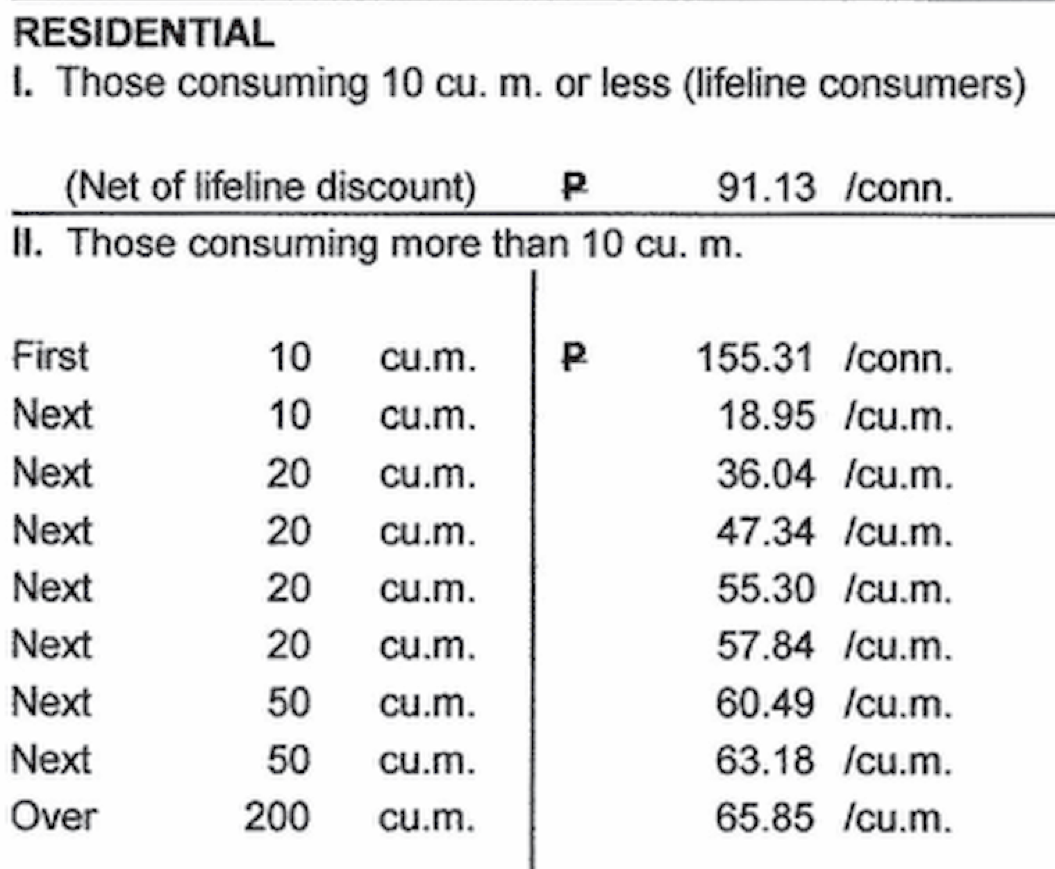
\includegraphics[scale=.8]{tables/tariff_pic_png.png} \\
% \footnotesize{``conn.'' refers to connection, ``cu.m.'' refers to cubic meters of usage \\ per month, and \textbf{P} refers to Philippine Pesos.  Includes Tariff as of February, 2019.}
% \end{center}
% \end{figure}


\begin{table}[H]
\centering
\caption{Example Residential Tariff As Presented to Consumers}\label{table:tarifftrue}
\vspace{-2mm}
\begin{tabular}{l*{1}{r}}
\toprule
Usage (m3) & Price (PhP) \\
\midrule
Under  10    &   104.12/conn. \\
Over  10     &   180.35/conn. \\
Next   10    &   19.20/cu.m. \\
Next    20   &   25.32/cu.m. \\
Next   20    &   33.21/cu.m. \\
Next    20   &   40.73/cu.m. \\
Next    20   &   45.92/cu.m. \\
Next    50   &   48.86/cu.m. \\
Next   50    &   55.31/cu.m. \\
Over  200    &   57.60/cu.m. \\
\bottomrule
\multicolumn{2}{l}{\scriptsize Mean tariff 2010-2015 with value added tax. }\\[-.5em]
\multicolumn{2}{l}{\scriptsize ``conn.'' refers to connection. }\\[-.5em]
\multicolumn{2}{l}{\scriptsize ``cu.m.'' refers to m3/month.  50 PhP$\sim$1 USD }
\end{tabular}
\end{table}

Table~\ref{table:tarifftrue} provides the monthly tariff structure as it is presented to consumers.  Consumers face a fixed price as well as marginal prices for any usage above 10 m3.  The regulator gradually adjusts prices at roughly yearly intervals in order to ensure that the utility is able to exactly cover its costs.  The marginal price is highly non-linear, accelerating quickly at low usage levels before slowly increasing at high usage levels.  To achieve a tractable approximation of this price schedule, Table~\ref{table:tcd_predict} fits a simple regression model predicting average price as a function of an intercept, $p_1$, and monthly usage levels, $p_2$.  This model predicts that a increase in monthly usage of 10 m3 results in an increase in average price of 2.2 PhP/m3.  

\begin{table}[H]
\small
\centering
\caption{Average Price and Monthly Usage}\label{table:tcd_predict}
\vspace{-2mm}
\begin{tabular}{lc}
\toprule
& \small Avg. Price: $\frac{\text{Bill (PhP)}}{\text{Usage (m3)}}$    \\
\midrule 
Usage (m3)          &        0.29\textsuperscript{a}\\
                    &      (0.00)                   \\[0.5em]
Intercept           &       17.53\textsuperscript{a}\\
                    &      (0.05)                   \\[0.5em]
Household-Months    &   1,946,309                   \\

\bottomrule
\multicolumn{2}{l}{\scriptsize \textsuperscript{c} p$<$0.10,\textsuperscript{b} p$<$0.05,\textsuperscript{a} p$<$0.01 }
\end{tabular}
\end{table}



\subsection{Stayer Descriptives}\label{appendix:stayerdescriptives}


\begin{table}[H]
\centering
\caption{Descriptives for Stayers}\label{table:descriptives_stayers}
\vspace{-2mm}
\begin{tabular}{l*{1}{cccccc}}
\toprule
 & Mean & SD & Min & 25th & 75th & Max  \\
\midrule
 Usage (m3)  & 30.0  & 20.5  & 0.0  & 17.0  & 38.0  & 200.0  \\ 
 Bill  & 931  & 1,269  & -4,862  & 323  & 1,122  & 78,409  \\ 
 Unpaid Balance  & 3,009  & 5,953  & -4,995  & 330  & 3,016  & 79,959  \\ 
 Share of Months with Payment  & 0.62  & 0.49  & 0.00  & 0.00  & 1.00  & 1.00  \\ 
 Payment Size  & 1,448  & 1,769  & 0  & 500  & 1,753  & 76,029  \\ 
 Days Delinquent  & 90.9  & 161.8  & 0.0  & 0.0  & 91.0  & 720.0  \\ 
 Delinquency Visits per HH  & 1.35  & 0.63  & 1.00  & 1.00  & 2.00  & 6.00  \\ 
 Share of Months Disconnected  & 0.04  & 0.19  & 0.00  & 0.00  & 0.00  & 1.00  \\ 

\bottomrule
\multicolumn{7}{c}{Total Households: 11,856  Obs. per Household: 61.8 Total Obs.: 731,935}
\end{tabular}
\end{table}

\begin{figure}[H]
\centering
\caption{Stayers Share of Households that Receive a Delinquency Visit \\ depending on Days Delinquent in the Previous Month}\label{figure:dc_hazardstayers}
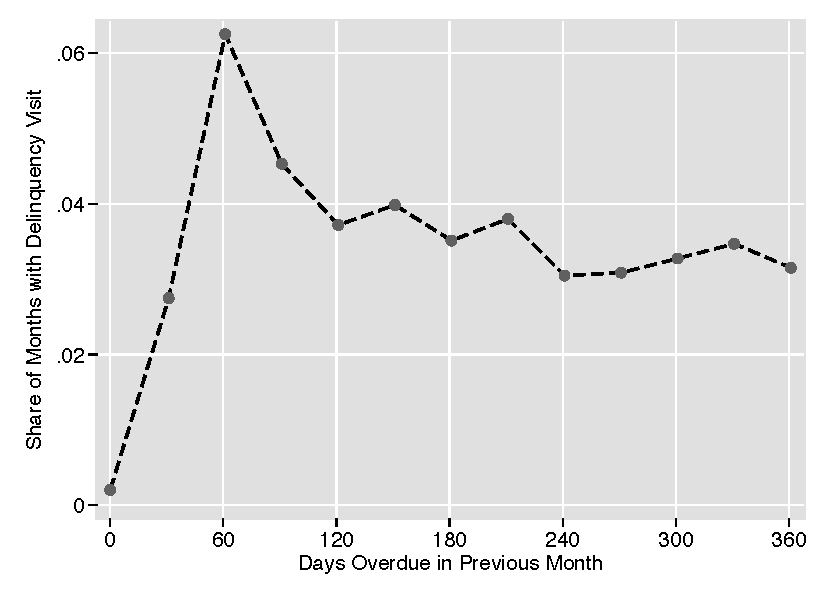
\includegraphics[scale=.7]{tables/connected_visit_hazard.pdf} \\
{ \footnotesize Only stayer households. }
\end{figure}

% \subsection{Discussion of the Discount Rate}


\subsection{Usage Before Permanent Disconnection}\label{appendix:permanentdc}

%%% DISCUSS AVERAGE LENGTH OF ACCOUNTS IN THE SAMPLE!!!

Figure~\ref{figure:dc_permanent} plots average usage across households according to the number of months before these households permanently disconnect. Average consumption increases in the months leading up to permanent disconnection.  This increase is likely due to some households using water as if they faced a zero marginal price since they know that they will never pay their bills.  With an average bill of 691.6PhP/month, leaving an outstanding balance of 7,119PhP at permanent disconnection is equal to enjoying an average of around 18 months of free water consumption.

\begin{figure}[H]
\centering
\caption{Average Usage in Months Before Permanent Disconnection}\label{figure:dc_permanent}
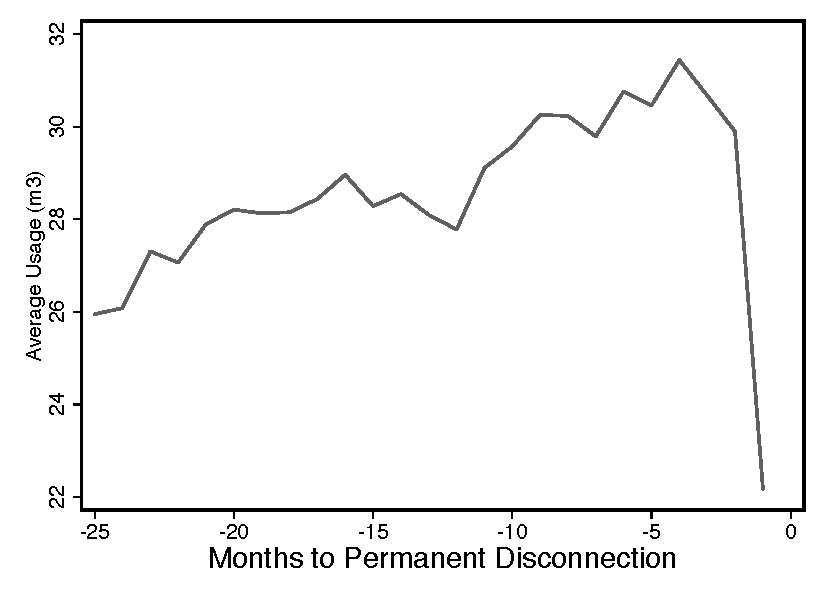
\includegraphics[scale=.7]{tables/line_disc_graph.pdf} \\
{ \footnotesize Negative months indicate months before permanent disconnections. }
\end{figure}





% \subsection{Sampling of the Connection Survey}\label{appendix:pawssampling}

% Connection survey documentation indicates that surveyors used stratified sampling where the number of connections surveyed was proportional to the census population in each small administrative district (Barangay).  Surveyors randomly interviewed owners of connections until reaching these targets.  


% Although this approach ensures that connections are randomly sampled within areas, it may also lead to oversampling of areas with few connections.  To measure the extent of possible oversampling, the following regression expresses the share of surveyed connections in each Meter Reading Unit (MRU) --- the water company's smallest unit of geography including around 200 households per unit on average --- as a function of the demographics of households owning connections, $Z_{MRU,i}$, in each of these MRUs:

% To test this hypothesis, the following equation predicts the share of connections surveyed in each Meter Reading Unit (MRU) --- the smallest geographical unit used by the water provider including a couple hundred water connections on average --- according to demographics of households owning connections, $Z_{MRU,i}$, in each of these MRUs:
% \begin{align*}
% ShareSurveyed_{MRU} = \beta Z_{MRU,i} + \epsilon_{MRU,i}
% \end{align*}
% Table~\ref{table:pawssampling} provides the results for this regression.  Although many coefficients are statistically significant consistent with large sample sizes for this estimation, the magnitudes of the effects are small in economic terms across most measures.  For example, increasing the average number of households per connection by a standard deviation (0.65) results in a 0.0021 percentage point decrease in the probability of being surveyed; given a mean survey probability of 6 percentage points, this change represents only a 3.3 percent decrease.  Dwelling types are the strongest predictor of coverage, indicating that surveyors may have oversampled apartments possibly due to easier availability to survey.  Taken together, these results suggest that to the extent that non-random sampling may affect results, it will lead to an underestimation of the importance of sharing networks in Manila.

% \begin{table}[H]
% \centering
% \caption{ Predicting Share of Connections Surveyed with \\ Connection Owner Demographics }\label{table:pawssampling}
% \begin{tabular}{lc} \hline
 & (1) \\
VARIABLES & Percent Surveyed \\ \hline
 &  \\
Mean Consumption (m3) & 0.000286*** \\
 & (3.94e-05) \\
HHs per Connection & -0.00334*** \\
 & (0.000775) \\
HH Size & -0.000285 \\
 & (0.000190) \\
Age HoH & 0.000138*** \\
 & (2.27e-05) \\
Total Empl. & 4.04e-05 \\
 & (0.000326) \\
Low Skill Emp. & 0.00158* \\
 & (0.000909) \\
Apartment & 0.00704*** \\
 & (0.00157) \\
Single House & -0.0114*** \\
 & (0.00117) \\
Constant & 0.117*** \\
 & (0.00250) \\
 &  \\
Observations & 45,907 \\
R-squared & 0.018 \\
Mean Coverage & .06 \\
Std. Dev. Coverage & .06 \\
 Cluster MRU & Yes \\ \hline
\multicolumn{2}{c}{ Robust standard errors in parentheses} \\
\multicolumn{2}{c}{ *** p$<$0.01, ** p$<$0.05, * p$<$0.1} \\
\multicolumn{2}{c}{ 2,947 Meter Reading Units (MRUs)} \\
\end{tabular}

% \end{table}

\nocite{*}
\singlespacing
\setlength{\bibsep}{7pt}
\bibliographystyle{abbrvnat}
\bibliography{ref}



\end{document}


